\documentclass[a4, english]{article}

%Import from a relative path
\usepackage{import}
\usepackage{framed}
\import{../../LaTeX-Preamble/}{preamble_dk.tex}

\settitle{Eksamensnoter}{Machine Learning}

\definecolor{lstKey2}{rgb}{0,0,0}
\lstset{xleftmargin= .1\textwidth,
  xrightmargin= .1\textwidth,
  frame=none
}

\author{Martin Nørskov Jensen}

\begin{document}

\maketitle

\newpage    
\tableofcontents
\newpage

\section{Linear Models}
\subsection{Disposition}
\begin{enumerate}
	\item Linear regression 
  \begin{itemize}
  	\item The problem
    \item The model
    \item Algorithm
  \end{itemize}
  \item Logistic regression
  \begin{itemize}
  	\item The problem 
    \item The model
    \item Error measure
    \begin{itemize}
    	\item Finding gradient
    \end{itemize}
    \item Gradient Descent
    \begin{itemize}
    	\item Standard GD
      \item SGD
      \item Minibatch SGD
    \end{itemize}
  \end{itemize}
  \item Nonlinear Transform
  \begin{itemize}
  	\item Why is it useful
    \item Definition 
    \item Generalization and computation issues
  \end{itemize}
\end{enumerate}
\newpage
\subsection{Linear regression}
\begin{itemize}
  \item Linear regression tries to find the based line that fits all the points in the dataset
	\item Linear regression algorithm is based on minimizing the squared error between $h(x)$ and $y$ 
\begin{equation*}
  E_\text{out}(h) = \mathbb E[(h(\pmb x) - y)^2]
\end{equation*}
  \item The expected value is taken with respect to the joint probability distribution $P(x,y)$ 
  \item The in-sample error is computed as 
\begin{equation*}
  E_\text{in}(h) = \frac{1}{n}\sum_{n=1}^N(h(\pmb x_n) - y_n)^2
\end{equation*}
  \item $h$ takes the form of a linear combination of the components of $x$ i.e 
\begin{equation*}
  h(\pmb x) = \sum_{i=0}^dw_ix_i = \pmb w^T\pmb x
\end{equation*}
  \item	where $x_0 = 1$ an $\pmb x \in \{1\} \times \mathbb R ^d$ as usual and $\pmb w \in \mathbb R^{d+1}$ 
  \item $X \in \text{Mat}_{(n, d+1)}(\mathbb R)$ is the data matrix where the inputs $x_i$ is as row vector for $i=1,\dots, n$
  \item $\pmb y \in \mathbb R^N$ is the target vector where components are the target values $y_i$ for $i=1,\dots, n$ 
  \item Linear regression algorithm
  \begin{enumerate}
  	\item Construct the matrix $X$ and the target vector $\pmb y$ from the data set $((\pmb x_1, y_1), \dots, (x_n,y_n))$ where each $\pmb x$ includes the $x_0=1$ bias coordinate as follows
\begin{equation*}
  X = 
  \begin{pmatrix} 
    - & \pmb x_1^T & - \\
    - & \pmb x_2^T & - \\
      & \vdots & \\
    - & \pmb x_n^T & - \\
  \end{pmatrix}
  , \pmb y = \quad
  \begin{pmatrix} 
  y_1 \\ y_2 \\ \vdots \\ y_n
   \end{pmatrix}
\end{equation*}
    \item Compute the pseudo-inverse $X^\dagger$ of the matrix $X$. If $X^TX$ is invertible
\begin{equation*}
  X^\dagger = (X^TX)^{-1}X^T
\end{equation*}
    \item Return $\pmb w_{\text{lin}} = X^\dagger \pmb y$ 
  \end{enumerate}

\end{itemize}


\subsection{Logistic regression}
\begin{itemize}
	\item In logistic regression one is trying to learn the target function
\begin{equation*}
  f(\pmb x) = \mathbb P[y = +1 \mid \pmb x]
\end{equation*}
  \item The sigmoid function $\sigma$ is used to predict something between 0 and 1 
\begin{equation*}
    \sigma(s) = \frac{1}{1+e^{-s}}
\end{equation*}
  \begin{itemize}
  	\item The output can be interpreted as the probability for a binary even
    \item It is refereed to as a soft threshold instead of the hard threshold in classification
    \item To use a hard threshold in classification using this model the one with the highest probability is chosen 
    \item It is also called the \textbf{logistic function}
  \end{itemize} 
  \item The logistic model is the following 
\begin{equation*}
  h(\pmb x) = \sigma (\pmb w^T \pmb x )
\end{equation*}
  \item The probabilities is as follows
\begin{equation*}
	P(y \mid x,w) = 
		\begin{cases}
			\mbox{$\sigma(w^Tx)$} & \mbox{if $y=1$} \\
			\mbox{$1-\sigma(w^Tx)$} & \mbox{if $y=0$} \\
		\end{cases}
\end{equation*}

\end{itemize}

\subsubsection{Error measure}
\begin{itemize}
	\item The error measure used is based on how likely it is that we get this output $y$ from our input $\pmb x$ 
  \item To define the error measure maximum likelihood is used 
  \begin{itemize}
    \item $P(D \mid w)$ is the following
\begin{equation*}
  P(D \mid w) = \prod_{i=1}^nP(y_i \mid x_i,w) = \prod_{i=1}^n \sigma(w^Tx)^T(1-\sigma(w^Tx))^{1-y}
\end{equation*}
    \item The negative log likelihood is the following
\begin{equation*}
  \text{NLL}(D \mid w) = - \sum_{i=1}^n y\ln(\sigma(w^TX)) + (1-y)\ln(1- \sigma(w^Tx))
\end{equation*}
    \item The in sample error is defined as 
\begin{equation*}
  E_{in}(w) = \frac1n \text{NLL}(D \mid w)
\end{equation*}
    \end{itemize}
  \item To minimize the in sample error we want to compute the derivative 
  \begin{itemize}
  	\item We define the following parts of the error for a single point
\begin{align*}
  s &= w^Tx \\
  p &= \sigma (s) \\
  l_1 &= \ln p \\
  l_2 &= \ln (1-p) \\
  o_1 &= -y \cdot l_1  \\
  o_2 &= -(1-y) \cdot l_2 \\
  cost &=  o_1 + o_2 
\end{align*}
  \newpage % TODO slet
    \item The gradients for the different parts of the equation is then calculate
\begin{align*}
   J_{cost,o_1} &= 1 \\ 
   J_{cost,o_2} &= 1 \\
  J_{o_1, l_1} &= -y \\
  J_{o_2, l_2} &= -(1-y) \\
    J_{l_1, p} &= \frac{1}{p}  \\
    J_{l_2, p} &= -\frac{1}{1-p} \\
    J_{p, s} &= \sigma(s)(1- \sigma(s)) \\
    J_{s, w} &= x^T \\
\end{align*}
  \item The gradients for the subelements is then used to calculate the gradient for the whole thing
\begin{align*}
  J_{cost,w} &= 1 \cdot (-y) \frac1p \sigma(s)(1- \sigma(s)) \cdot x^T + 1 \cdot -(1-y) \frac{1}{1-p} \cdot  \sigma(s)(1- \sigma(s)) \cdot x^T \\
            &= -y \frac1{\  \sigma(s)} \sigma(s)(1- \sigma(s)) \cdot x^T + -(1-y) \frac{1}{1- \sigma(s)} \cdot  \sigma(s)(1- \sigma(s)) \cdot x^T \\
            &= -y (1- \sigma(s)) \cdot x^T + (1-y) \sigma(s) \cdot x^T \\
            &= -y \cdot x^T + \sigma(s) \cdot x^T \\
            &= -x^T(y-\sigma(w^Tx)) \\    
\end{align*}
  \item To get the sum of all the gradients the following products is used
\begin{equation*}
  - X^T(Y-\sigma(Xw))
\end{equation*}

\end{itemize}

\end{itemize}

\subsubsection{Gradient Descent}
\begin{itemize}
	\item To minimize the error function using the gradient gradient descent is used
  \begin{itemize}
  	\item This is done since one cannot analytically set the gradient equal to zero and solve for the best values of $w$ 
  	\item You start somewhere and go the steepest way down the surface
    \item The minimum that it finds is guaranteed to be an optimal if the given function is convex  
  \end{itemize}
  \item It is done by iterative taking the subtracting the negative gradient multiplied by some learning rate until some stopping criterion is med
  \begin{itemize}
  	\item It is important to chose a good learning rate 
    \item A too small learning rate will have too small improvements in each step and will therefore result in the minimum never being reached
    \item A too high error rate will result in overshooting the goal and maybe increasing the error function
    \item $\eta_t = \eta || \bigtriangledown E_\text{IN} ||$ is typically chosen to obtain a good variable step size   
  \end{itemize}
  \item Psuedo code for Gradient Descent
\begin{lstlisting}[mathescape=true, keywordstyle=\ttfamily]
$w$ = randomly or smart chosen vector
$\eta=0.1$ 
for $i=1$ to $100$ 
  $w=w--\eta \nabla E_{\text{in}}(w)$
\end{lstlisting} 
  \item The problem with gradient descent is that computing the gradient takes $O(n)$ time 
  \begin{itemize}
  	\item This is long time for moving a small step
  \end{itemize}
\end{itemize}

\subsubsection{Stochastic Gradient Descent}
\begin{itemize}
  \item SGD is often used instead of GD 
  \begin{itemize}
  	\item It only computes the gradient for a single point
    \item Much faster that GD 
  \end{itemize}
  \item Psuedo code for stochastic gradient descent
\begin{lstlisting}[mathescape=true, keywordstyle=\ttfamily]
$w$ = randomly or smart chosen vector
$\eta=0.1$ 
for $i=1$ to $100$ 
  Pick $(x_i,y_i) \in D$ uniformly at random and use
  $w=w--\eta \nabla$loss$(h_w(x_r), y_r)$ 
\end{lstlisting} 
  \item It uses more iterations that GD but it is cheaper
  \item It may take sublinear time 
  \item It gets on average the same gradient
  \item Has a large variance i.e. is noisy 
\end{itemize}

\subsubsection{Mini-Batch SGD}
\begin{itemize}
	\item Mini-Batch SGD takes a mini batch of size $b$ and computes the average gradient it
  \item It has the same correct expectation but less variance the standard SGD 
  \item Psuedo code
\begin{lstlisting}[mathescape=true, keywordstyle=\ttfamily]
$w$ = randomly or smart chosen vector
$\eta=0.1$ 
for $i=1$ to $100$ 
  Randomly shuffle data 
  Split data into disjoint minibatches $b_1, \dots, b_{n/d}$ of size $b$ by grouping $b$ consecutive elements repeatedly 
  for $j=1$ to $n/b$ 
    $w=w--\eta \nabla$loss$(h_w(x_r), y_r)$ 
\end{lstlisting} 
\end{itemize}

\subsection{Nonlinear Transform}
\begin{itemize}
	\item A nonlinear transform can be used to transform non linear separable data into data that is
  \begin{itemize}
  	\item The space $\mathcal Z$ that is generated is called \textbf{the feature space}
    \item The transformation from the original space $\mathcal X$ to $\mathcal Z$ is called a \textbf{feature transform}
  \end{itemize}
    \item Any linear hypothesis $\tilde h$ in $\pmb z$ corresponds to a (possible nonlinear) hypothesis of $\pmb x$ given by $h(\pmb x) = \widetilde{h} (\theta(\pmb x))$ where $\theta$ is a non linear transform
  \begin{itemize}
   	\item The set of these hypothesis is denoted by $\mathcal H_\theta$
  \end{itemize}
  \item The feature transform $\theta_Q$ is defined for degree-$Q$ curves in $\mathcal X$
  \begin{itemize}
  	\item It is called the Qth order polynomial transform
  \end{itemize}
  \item It may not be worth to insist on linear separability and use a feature transform
  \begin{itemize}
  	\item Sometimes it is better to tolerate a small $E_{in}$ than using a feature transform
    \item May result in overfitting
  \end{itemize}
  \item Computation is a problem since $\theta_Q$ maps a two dimensional vector $\pmb x$ to $\tilde d = \frac{Q(Q+3)}2$ dimensions which increases the computational cost
  \begin{itemize}
  	\item It only gets worse when starting from higher dimensions
  \end{itemize}
  \item The problem of generalization is an issue
  \begin{itemize}
  	\item There is a weaker gurantee that $E_{\text{OUT}}$ is small
  \end{itemize}

\end{itemize}

\newpage

\section{Learning Theory}
\subsection{Disposition}
\begin{enumerate}
	\item Generalization
  \begin{itemize}
  	\item Dichotomy
    \item Growth function
    \begin{itemize}
    	\item Definition
      \item Break point
    \end{itemize}
  \item VC Dimension  
  \begin{itemize}
  	\item Definition
    \item Bound
  \end{itemize}
  \end{itemize}  
  \item Regularization
  \begin{itemize}
  	\item What is regularation?
    \begin{itemize}
    	\item Avoid overfitting
      \item Minimizing model complexity
    \end{itemize}
    \item Weight decay
    \begin{itemize}
    	\item Augmented error
      \item Regularization and $n$ 
      \item Picking $\lambda$ importance 
    \end{itemize}
  \end{itemize}
  \item Validation 
  \begin{itemize}
  	\item Estimation of $E_\text{out}$ 
    \item Validation set
    \begin{itemize}
    	\item How is it created
      \item How is it used ($E_\text{val}$)      
    \end{itemize}
    \item Model selection
  \end{itemize}
\end{enumerate}
\newpage

\subsection{Generalization}
\begin{itemize}
	\item The \textbf{generalization error} is the difference between $E_{\text{in}}$ and $E_\text{out}$ 
  \begin{itemize}
  	\item \textbf{Hoeffding Inequality}, provides a way to characterize it with a probabilistic bound 
    \item The Inequality can be rephrased as follows: pick a tolerance level $\delta$ such as 0.05 and assert with probability at least $1-\delta$ that
\begin{equation*}
  E_\text{out}(g) \leq E_\text{in}(g) + \sqrt{\frac1{2N} \ln \frac{2M}\delta} 
\end{equation*}
    This is refereed to as the generalization bound, where $N$ is the number of data points and $M$ is the number of hypotheses

  \end{itemize}
  \item \textbf{Definition} Let $x_1, \dots, x_N \in \mathcal X$. The \textbf{dichotomies} generated by $\mathcal H$ on these points are defined by
\begin{equation*}
  \mathcal H (\pmb x_1, \dots, \pmb x_N )= \{ (h(\pmb x_1), \dots, h(\pmb x_N )) \mid h \in \mathcal H \} 
\end{equation*}
  \item \textbf{Definition} The \textbf{growth function} is defined for a given hypothesis set $\mathcal H$ by 
\begin{equation*}
  m_\mathcal{H}(N) = \underset{\pmb x_1, \dots, \pmb x_N \in \mathcal X}{\text{max}} | \mathcal H(\pmb x_1, \dots, \pmb x_N)|
\end{equation*}
 $| \cdot |$ denotes the number of elements in the set 
  \item It is said that an $\mathcal H$ can \textbf{shatter} $\pmb x_1, \dots, \pmb x_N$  if the $\mathcal H$ is as diverse as it can be on this particular sample
  \item \textbf{Definition} If there is no data of size $k$ that can be shattered by $\mathcal H$, then $k$ is said to be a \textbf{break point} for $\mathcal H$ 
  \begin{itemize}
  	\item If $k$ is a break point, then $m_{\mathcal H}(k)<2^k$ 
  \end{itemize}
  \item \textbf{Definition} The \textbf{VP dimension} of a hypotheses set $\mathcal H$ denoted by $d_{vc}(\mathcal H)$ or $d_{vc}$ is the largest value of $N$ for which $m_{\mathcal H}(N)=2^N$
  \begin{itemize}
  	\item If $m_\mathcal H (N) = 2^N$ for all $N$, then $d_{vc}(\mathcal H) = \infty$.
    \item There are no smaller breakpoint than $k=d_{vc}+1$ 
    \item The VC dimension of a $d$ dimensional perceptron is $d+1$. 
  \end{itemize}
  \item \textbf{Theorem} VC generalization bound. For any tolerance $\delta > 0$ 
\begin{equation*}
  E_\text{out}(g) \leq E_\text{in}(g) + \sqrt{\frac8N\ln\frac{4m_\mathcal{H}(2N)}\delta}
\end{equation*}
with probability $\geq 1- \delta$  
  \begin{itemize}
  	\item It is a quite loose bound, since it is independent of the training algorithm
    \item Models with lower $d_{vc}$ tend to do better than the ones with higher $d_{vc}$
    \item The following inequality is true between the VC dimension and the growth function
\begin{equation*}
  m_{\mathcal H}(N) \leq N^{d_vc}+1
\end{equation*}

    \item The second part is often called the penalty and denoted in the following way 
\begin{equation*}
  \Omega(N,\mathcal H, \delta) = \sqrt{\frac8N\ln\frac{4((2N)^{d_\text{vc}} + 1)}\delta}  
\end{equation*}
  \end{itemize}  
\end{itemize}

\subsection{Regularization}
\begin{itemize}
	\item Regularization is a way to combat overfitting i.e.~picking a lower $E_\text{in}$ that results in a higher $E_\text{out}$ 
  \begin{itemize}
  	\item $E_{\text{in}}$ is not a good guide alone for learning 
    \item A typical case of overfitting is having a complex model i.e. a model with a large VC dimension which uses its extra degrees of freedom to learn the noise 
    \item It can be thought of as trying to minimize the model complexity penalty $\Omega(H)$ instead of just $E_\text{in}$ 
    \item Constraints the learning algorithm to use simpler hypotheses
    \item No regularizer will be ideal for all settings
  \end{itemize}
  \item A type of regularization is known as known as \textbf{weight decay} 
  \begin{itemize}
  	\item The \textbf{augmented error} function is defined as 
    \begin{equation*}
      E_\text{aug}(\pmb w) = E_\text{in}(\pmb w) + \lambda ||w||^2
    \end{equation*}
    where $\lambda \geq 0$ is a free parameter
    \item This methods enforces the trade-off between making the in-sample error small and the weights small 
    \item The idea is that larger weights allows for more complicated models
    \item The need for regularization goes down as the number of data points goes up
    \item The \textbf{augmented error} is in general for a hypothesis set $h \in \mathcal H$
\begin{equation*}
    E_\text{aug}(h,\lambda,\Omega) = E_\text{in}(h) + \frac\lambda N \Omega(h)
\end{equation*}
    where for weights decay $\Omega(h) = \pmb w^T\pmb w$
    \item It is important to pick the right $\lambda$
  \end{itemize}

\end{itemize}

\subsection{Validation}
\begin{itemize}
	\item Validation tries to estimate out-of-sample error directly
 	\item Validation uses a \textbf{validation set} which is a subset of the data that is removed before training
  \begin{itemize}
  	\item It will be used to make a choice in the learning process and is therefore not a test set  
  \end{itemize}
  \item The validation set is created an used in the following way
  \begin{enumerate}
     \item It is created by partitioning the data into a training set $\mathcal D_{\text{train}}$ of size $N-K$ and a validation set $\mathcal D_{\text{train}}$ of size $K$ 
    \item The training data is used in the learning algortihm and a final hypthesis $g^- \in \mathcal H$ is found 
    \item The validation error $E_\text{val}(g^-)$ is computed by taking the point wise error over the training set 
\begin{equation*}
  E_\text{val}(g^-)=\frac1K\sum_{\pmb x_n \in \mathcal D_\text{val}} e(g^-(\pmb x_n),y_n)
\end{equation*}
  \end{enumerate}
  \begin{itemize}
  	\item It is important to choose a good $K$ for $E_\text{val}$ to be a good estimator of $E_\text{out}$ 
    \begin{itemize}
      \item $K$ is often chosen to be $\frac N5$ 
    \end{itemize}
  \end{itemize}
  \item One should not output $g^-$ we should output $g$ which is trained on the entire hypothesis set $D$
  \begin{itemize}
  	\item To estimate $E_\text{out}$ we use that $E_\text{out}(g) \leq E_\text{out}(g^-)$ because of the learning curve
  \end{itemize}
  \item Validation can be used for model selection i.e. given a $M$ models $\mathcal H_1, \dots, \mathcal H_M$ which one is best
  \begin{itemize}
  	\item The training set $\mathcal D_\text{train}$ is used to learn the final hypothesis $g^-_m$ for each model
    \item The validation error is found on each of the models 
    \item The model with the lowest validation error is chosen 
    \item This can be used to choose a good $\lambda$ for regularization
  \end{itemize}
\end{itemize}

\newpage

\section{Support Vector Machines}
\subsection{Disposition}
\begin{enumerate}
	\item Problem 
  \begin{itemize}
  	\item The data points
    \item The hyperplane parameters
    \item The desired result
  \end{itemize}
  \item Margins
  \begin{itemize}
  	\item Functional margin
    \item Geometric margin
  \end{itemize}
  \item Reducing problem
  \begin{itemize}
  	\item Define problem
    \item Scaling to pick functional margin 1
    \item Changing to minimization problem 
  \end{itemize}
  \item Lagrange
  \begin{itemize}
  	\item Problem
    \item Primal problem
    \begin{itemize}
    	\item Primal infeasible
      \item Primal feasible
    \end{itemize}
    \item Dual problem
    \begin{itemize}
    	\item Dual feasible
    \end{itemize}
    \item Relation ship between dual and primal
    \begin{itemize}
    	\item When are they equal 
      \item KKT Conditions 
    \end{itemize}
  \end{itemize}
  \item SVM in Dual form
  \begin{itemize}
  	\item Changing the problem
    \item Lagrangian of the problem 
    \item Reducing using KKT conditions 
    \item Solution an a way to compute this
    \item Relate to Kernels 
  \end{itemize}
\end{enumerate}
\newpage

\subsection{Problem}
\begin{itemize}
	\item The target $y$ is $\{-1,1\}$ 
  \item The hyperplane parameters are $w$ and $b$ 
  \item The hyperplane is $w^Tx+b=0$ 
  \begin{itemize}
  	\item The class is $1$ if $w^Tx+b \geq 0$ and if not it is $-1$ 
  \end{itemize}
  \item The data is $D=\{(x_1,y_1), \dots, (x_n,y_n)\}$ with $|D| = n$
  \item It is assumed that the data is linear separable 
  \item An SVM picks the hyperplane with the maximum distance to the closest points 
  \begin{itemize}
  	\item Since there are much fewer large margin hyperplane the found generalization should generalize better  
  \end{itemize}
\end{itemize}

\subsection{Margins}
\begin{itemize}
	\item Given a training example $(x_i, y_i)$ the \textbf{functional margin} of $(w,b)$ with respect to the training example is defined as follows 
\begin{equation*}
  \hat \gamma_i=y_i(w^Tx_i+b)
\end{equation*}
  \begin{itemize}
  	\item A large functional margin represents a confident and correct prediction
    \item Given a training set $S=\{(x_1,y_1), \dots, (x_n,y_n)\}$ the functional margin of $(w,b)$ with respect to $S$ is 
\begin{equation*}
  \hat \gamma = \min_i \hat \gamma_i
\end{equation*}
    \item A negative functional margin represents a misclassified point 
  \end{itemize}

  \item The \textbf{geometric margin} of $(w,b)$ with respect to a training set $(x_i, y_i)$ is defined to be
\begin{equation*}
	\gamma_i = y_i \Bigg( \bigg( \frac w{||w||} \bigg)^T x_i + \frac b{||w||}  \Bigg)
\end{equation*}
\begin{itemize}
  \item The following is true for the geometric and functional margin $\hat  \gamma = \frac{\hat \gamma_i}{||w||}$ 
	\item If $||w|| = 1$ the function margin equals the geometric margin 
  \item The geometric margin is not influenced by scaling 
  \begin{itemize}
  	\item This is important since if this was not the case one could scale $w$ by some number an obtain a large margin 
  \end{itemize}    
  \item Given a training set $S=\{(x_1,y_1), \dots, (x_n,y_n)\}$ the geometric margin of $(w,b)$ with respect to $S$ is 
\begin{equation*}
  \gamma = \min_i \gamma_i
\end{equation*}
\end{itemize}
  

\end{itemize}
\subsection{Reducing problem}
\begin{itemize}
	\item The problem of finding a decision boundary with the largest geometric margin is the following optimization problem 
\begin{equation*}
  \begin{split} 
    \max_{w,b}: \ &\min_i \frac{y_i(w^T x_i+b)}{||w||}\\
    \text{s.t.} \ & y_i(w^T x_i+b) \geq 0, \ i= 1, \dots, n \\
  \end{split}
\end{equation*}
  Here we are minimizing the geometric margin on a $w$ that classifies the data correctly 
  \item Since the scaling the parameters $w$, $b$ does not do anything to our solution we pick the one with functional margin $1$, which gives a new optimization problem
\begin{equation*}
  \begin{split} 
     \max_{w,b}: \ & \frac{1}{||w||}\\
    \text{s.t.} \ & y_i(w^T x_i+b) \geq 1, \ i= 1, \dots, n \\
  \end{split}
\end{equation*}
One knows that the smallest functional margin is 1 since if all margins is above we can find a better solution by scaling $w$ and $b$ down to get points with functional margin $1$ 
  \item The $||w||$ is the scaled and we change the problem to a minimizing problem 
\begin{equation*}
  \begin{split} 
     \min_{w,b}: \ & \frac12||w||^2\\
    \text{s.t.} \ & y_i(w^T x_i+b) \geq 1, \ i= 1, \dots, n \\
  \end{split}
\end{equation*}
  This is called the \textbf{optimal margin classifier} and is a convex problem
\end{itemize}

\subsection{Lagrange}
\begin{itemize}
	\item Given a problem of the following form
\begin{equation*}
  \begin{split} 
          \min: \ & f(x)\\
    \text{s.t.} \ & g_i(x) \leq 0, \ i=1,\dots,m\\
                  & h_i(x) = 0 , \ i=1,\dots,p\\
  \end{split}
\end{equation*}
  Let $x^*$ denote the optimal solution to the problem
  \item The Lagrangian is defined
\begin{equation*}
  \mathcal L(x,\alpha, \beta) = f(x) + \sum_{i=1}^m \alpha_ig_i(x) + \sum_{i=1}^p \beta_i h_i(x)
\end{equation*} 
  $\alpha, \beta$ are called \textbf{Lagrange multipliers}
  \item The following is the \textbf{Primal Problem}
\begin{equation*}
  Pr(x) = \max_{\alpha, \beta: \alpha \geq 0} \mathcal L (x,\alpha, \beta)
\end{equation*}
  	\item An input $x$ is \textbf{primal infeasible} if for some $i$, $g_i(x) >0$ or $h_i(x) \ne 0$ 
  \begin{itemize}
    \item $\Rightarrow Pr(x) = \infty$
    \item $g_i(x) > 0$ means that $\alpha_i g_i(x)$ is unbounded
    \item $h_i(x) \ne 0$ means that $\beta_i h_i(x)$ is unbounded
  \end{itemize}
  \item An input $x$ is \textbf{primal feasible} if $g_i(x) \leq 0$ and $h_i(x) = 0$ for all $i$ 
  \begin{itemize}
    \item $\Rightarrow Pr(X) = f(x)$ 
    \item Since $g_i(x) \leq 0$ for all $i$ this means that one can maximize over all $\alpha_i \geq 0$ 
    \item Since $h_i(x) = 0$ for all $i$ this means that $b_i$ is irrelevant
  \end{itemize}
  \item $p^* = \min_x Pr(x) = Pr(x^*)$ 	
  \item The following is the \textbf{dual problem} 
  \begin{equation*}
    \min_x \mathcal L (x, \alpha, \beta)
  \end{equation*}
  \item $\alpha, \beta$ is dual feasible is $\alpha_i \geq 0$ for all $i$ 
 	\item The dual problem lower bounds the primal problem 
  \item $d^* = \max _{\alpha,\beta: \alpha_i \geq0} Du(\alpha, \beta)$ 
  \item The two problems are equal and the problem is strictly feasible if $f,g_i$ are convex and $h_i$ is affine 
  \begin{itemize}
  	\item If this is the case then the complementary slackness property is true
    \begin{equation*}
      \forall i \ \alpha_i^*g_i(x^*) = 0 
    \end{equation*} 
  \end{itemize}
  \item The \textbf{KKT Conditions} are the following on $x^*$ which are primal optimal, $\alpha^*,\beta^*$ which are dual optimal and $p^*=d^*$  
\begin{align*}
  \nabla_x  \mathcal L(x^*,\alpha^*,\beta^*) = 0 &\quad \text{(Stationary)} \\
                    g_i(x_i^*)\leq 0 \ \forall i &\quad \text{(Primal feasibility)} \\
                      h_i(x_i^*) = 0 \ \forall i &\quad \text{(Primal feasibility)}\\
                   \alpha_i^* \geq 0 \ \forall i &\quad \text{(Dual feasibility)}\\
             \alpha_i g_i(x_i^*) = 0 \ \forall i &\quad \text{(Complementary slackness)}
\end{align*}

\end{itemize}

\subsection{SVM in Dual form}
\begin{itemize}
	\item First we change the form of the problem to get it on the form of problem the Lagrange multipliers are defined for 
\begin{align*}
    \min_{w,b}: \ & \frac12||w||^2\\
    \text{s.t.} \ & - y_i(w^T x_i+b) + 1 \leq 0, \ i= 1, \dots, n \\
\end{align*}
  it is done by multiplying by $-1$ and adding $1$ on both sides
  \item The Lagrangian for the problem is
\begin{equation*}
  \mathcal L (w,b,\alpha) = \frac12||w||^2 - \sum_{i=1}^n \alpha_i (y_i(w^T x_i +b) -1)
\end{equation*}
  \item To eliminate $w$ and $b$ from the equation the followingis needed  
\begin{align*}
  f(w) &= w^T x \quad \nabla_f = x \\
  g(w) &= \frac12 ||w||^2 \quad \nabla_g = w
\end{align*}
  \item The Lagrangian is then differentiate with respect to $w$ 
\begin{align*}
  \nabla_w  \bigg(\frac12||w||^2 - \sum_{i=1}^n \alpha_i (y_i(w^T x_i +b) -1)\bigg) &= w - \sum_{i=1}^n \alpha_i y_i x_i
\end{align*}
  \item We then solve for $0$ since the gradient must be stationary (first KKT Condition)
\begin{equation*}
  0 = w- \sum_{i=1}^n \alpha_i y_i x_i \iff w = \alpha_i y_i x_i
\end{equation*}
  \item The same is then done for $b$ 
\begin{align*}
  \nabla_b \bigg(\frac12||w||^2 - \sum_{i=1}^n \alpha_i (y_i(w^T x_i +b) -1)\bigg) &= -\sum_{i=1}^n\alpha_i y_i 
\end{align*}
  \item We then solve for $0$ 
\begin{equation*}
  0 = -\sum_{i=1}^n\alpha_i y_i  \iff \sum_{i=1}^n\alpha_i y_i = 0
\end{equation*}
  \item These results are then used to eliminate $w$ and $b$ from the problem. The first part of the equation is reduced 
\begin{align*}
  \frac12||w||^2 &= \frac12 w^Tw \\
                 &= \frac12 \bigg(\sum_{i=1}^n \alpha_i y_i x_i\bigg)^T \bigg(\sum_{i=1}^n \alpha_i y_i x_i\bigg)\\
                 &= \frac12 \sum_i^n \sum_j^n \alpha_i\alpha_jy_iy_jx_i^Tx_j
\end{align*}
  \item The second part of the equation is reduced 
\begin{align*}
  - \sum_{i=1}^n \alpha_i (y_i(w^T x_i +b) -1) &=  - \sum_{i=1}^n \alpha_i (y_i(\bigg(\sum_{j=1}^n \alpha_j y_j x_j\bigg)^T x_i +b) -1)\\
                                            &= - \sum_i^n \sum_j^n \alpha_i\alpha_jy_iy_jx_i^Tx_j - \sum_i^n \alpha_iy_ib + \sum_i^n \alpha_i \\
                                            &= - \sum_i^n \sum_j^n \alpha_i\alpha_jy_iy_jx_i^Tx_j + \sum_i^n \alpha_i
\end{align*}
  \item The two reduced parts of the equation is then combined
\begin{equation*}
  \frac12\sum_i^n \sum_j^n \alpha_i\alpha_jy_iy_jx_i^Tx_j - \sum_i^n \sum_j^n \alpha_i\alpha_jy_iy_jx_i^Tx_j + \sum_i^n \alpha_i =   \sum_i^n \alpha_i - \frac12 \sum_i^n \sum_j^n \alpha_i\alpha_jy_iy_jx_i^Tx_j
\end{equation*}
  This equation can be solved by Quadratic Programming by finding the best $\alpha$ vector or e.g. coordinate ascent
  \begin{itemize}
    \item The optimal $\alpha^*$ results in the optimal $w$ and $b$ 
  	\item From this result the weight vector $w$ can be computed using the formula
  \end{itemize}
  \item An $x_i$ is a \textbf{support vector} if it is on the margin  
  \item All the $x_i$ with a none zero language multiplier is a support vector, since
\begin{equation*}
  \alpha_i^* > 0 \rightarrow -y_i (w^{*^T}x_i + b^*) +1 = 0 \Rightarrow |w^{*^T}x_i + b^*| = 1
\end{equation*}
  and all support vectors has margin $1$ 
  \begin{itemize}
  	\item This means that the hyperplane can be described by the support vectors 
  \end{itemize}
  \item $b$ can be found by selecting a support vector $x_i$ an solving for $b$ 
\begin{equation*}
  y_i (w^{*^T}x_i + b^*) - 1 = 0
\end{equation*}
\end{itemize}
\newpage

\section{Neural Nets}
\subsection{Disposition}
\begin{enumerate}
	\item The feedforward network
  \begin{itemize}
    \item Definitions and goal
    \item Cost functions 
    \item Model
  \end{itemize}
  \item Backprobagation 
  \begin{itemize}
  	\item Forward probagation
    \item Backprobagation
    \item Chain rule
    \item Algorithm
  \end{itemize}
  \item Regularization
  \item Convolutional
  \begin{itemize}
  	\item Definition
    \item Convolutional operation
    \begin{itemize}
    	\item Definitions
      \item Examples 
    \end{itemize}
    \item Motivation
    \begin{itemize}
    	\item Sparse interaction
      \item Parameter sharing
      \item Equivalent representations 
    \end{itemize}
    \item Pooling
    \begin{itemize}
    	\item Stages
      \item Max pooling
    \end{itemize}
  \end{itemize}
\end{enumerate}-
\newpage 

\subsection{Feedforward Neural Network}
\begin{itemize}
	\item The goal of a feedforward network is to approximate some function $f$ 
  \begin{itemize}
  	\item It defines a mapping $\pmb y = f(\pmb x; \pmb \theta)$ and learns the valus of the parameters $\pmb \theta$ that gives the best function approximation
    \item It is called \textbf{feedforward} since information flow through the function through intermediate computations and in the end output $\pmb y$
    \item It is composed of functions called \textbf{layers} where the final layer is the output layer
    \item The training data does no say what the inner layers should do
    \begin{itemize}
    	\item That is the job of the training algorithm
      \item They are called \textbf{hidden layers} 
    \end{itemize}
    \item The \textbf{width} of the model is the dimensionality of the hidden layers
    \item The \textbf{depth} is the overall amount of layers
    \item The neural network can be described by a DAG where each node is a neuron with multi inputs and a single output 
  \item \textbf{Universal Representor Theorem} Neural networks are universal representors
    \begin{itemize}
      \item For any function there exists a network large enough to achieve any degree of accuracy of approximation 
    	\item A one layer neural network is enough to describe any function 
    \end{itemize}
  \end{itemize} 
  \item Cost functions for neural networks  
  \begin{itemize}
  	\item They are more of less the same as those for the linear models such as 
    \item The total cost function used to train a neural network will often contain a regularization term 
    \item Most neural networks are trained using negative log likelihood
    \begin{itemize}
    	\item The advantages is that there is no need to design a cost function of each model 
      \item Specifying the model determines the cost function $\log p(\pmb y \mid \pmb x)$ 
    \end{itemize}
    \item The error function is neural networks is no longer convex
    \begin{itemize}
    	\item We can not be sure that we found the best solution only a local minima
      \item The parameters for the neural network is chosen at random to try and combat this 
    \end{itemize}
  \end{itemize}
  \item The model of a neural network is as follows 
  \begin{itemize}
  	\item A layer $i$ is represented as a weight matrix $W^{(i)}$ and a bias vector $b^{(i)}$  
    \item A layer $i$ has some activation function $g^{(i)}(z)$  
    \begin{itemize}
    	\item Activation functions should in general be differentiable
      \item But they do not need to bee differentiable everywhere e.g. the relu function  
    \end{itemize}
    \item Examples of activation functions
    \begin{itemize}
    	\item $reul(z) = \max\{0,z\}$
      \item $\sigma(z) = \frac1{1-e^{-x}} $
      \item $\tanh(z)$ 
    \end{itemize} 
    \item The ith layer in a neural network is calculated as follows
\begin{equation*}
  h^{(i)} = g^{(i)}(W ^{(i)T}\pmb h^{(i-1)} + \pmb b^{(i)})
\end{equation*}
  where the first layer uses $\pmb x$ instead of $h^{(i-1)}$  
  \end{itemize}
\end{itemize}

\subsection{Backpropagation}
\begin{itemize}
  \item \textbf{Forward propagation} is when the inputs $\pmb x$ provide initial information which then propagate up to the hidden units at each layer and then finally provides an output $\hat{\pmb y}$ 
  \begin{itemize}
  	\item In the end it computes a scalar cost $J(\pmb \theta)$ 
  \end{itemize}   
  \item The \textbf{backprobagation} algorithm allows the information from the cost to flow backward and then to compute the gradient for each layer 
  \begin{itemize}
  	\item This is used to compute the gradient, another algorithm is used to do the learning e.g. stochastic gradient descent 
    \item Often called the automatic chainrule 
  \end{itemize}
  \item To compute the gradients for the different layers the chain rule it used 
  \begin{itemize}
  	\item In vector notation the chain rule is written as 
\begin{equation*}
\nabla_{\pmb x}z = (\frac{\partial \pmb y}{\partial \pmb x})^T \nabla_{\pmb y} z
\end{equation*}
  where $\frac{\partial \pmb y}{\partial \pmb x}$ is the $n \times m$ Jacobian matrix of $g$ 
  \item The backpropagation algorithm consists of performing Jacobian-gradient product given the chain rule for each operation in the graph 
  \end{itemize}
  \item The following notation is used for the different parts of a neural network  
  \begin{itemize}
    \item $w_{ji}^l$ is the weight from neuron $i$ in layer $l-1$ to neuron $j$ in layer $l$
    \item $a_j^1 = x_j$ 
    \item $s_j^l=\sum_ia_i^{l-1}w_{j,i}^{l-1}+b_j^{l-1}$ 
    \item $a_k^l = \Phi(s_k^l)$
    \item $\delta_j^l=\frac{\partial e}{\partial s_j^l}$ 
  \end{itemize} 
  \item The following is the classic backpropagation algorithm 
\begin{lstlisting}[mathescape=true]
  Initialize weights $w^l_{i,j},b_j^l$ randomly
  // Forward propagation 
  $a_j^1 = x_j$
  for $l = 2 \rightarrow L$ 
    $s_j^l=\sum a_i^{l-1}w_{j,i}^{l-1} + b_j^{l-1} $
    $a_j^l = \Phi(s_j^l)$ 
  
  // Backpropagation 
  $\delta_j^L = \frac{\partial e}{\partial s_j^L}$
  for $l = L-1 \rightarrow 1$ 
    $\delta_j^l = \sum_{i=1}^{d_l+1}\delta_i^{l+1}w^l_{j,i}\frac{\partial \phi (s_j^l)}{\delta s_j^l}$
  
  // Output
  $\frac{\delta e}{\delta w_{j,i}^{l-1}} = a_i^{l-1}\delta_j^l \ $ $\frac{\partial e}{\partial b_j^{l-1}} = \delta_j^l$    
\end{lstlisting}
\end{itemize}

\subsection{Regularization}
\begin{itemize}
	\item Weight decay
  \begin{itemize}
  	\item $\lambda \cdot \sum_{l=1}^L ||W^{(l)}||$ is added to the error function
    \item Makes sure that the weights do not become to complicated  
  \end{itemize}
  \item Early stopping
  \begin{itemize}
  	\item A validation set is used
    \item When the no longer is any improvements in the validation error then stop the training
  \end{itemize}
  \item Dropout
  \begin{itemize}
  	\item Before each minibatch drop a neuron randomly with probability p i.i.d
    \item This averages existentially many models
    \item Forces the hidden units to be robust 
  \end{itemize}
\end{itemize}

\subsection{Convolutional Networks}
\begin{itemize}
	\item \textbf{Convolutional Networks} are a specialized kind of neural network for processing data that has a grid-like toplogy
  \begin{itemize}
  	\item A convolution is a specialized kind of linear operation
    \item They are neural networks where the use convolution in place of matrix multiplication it at least one of their layers 
  \end{itemize}  
\end{itemize}
  
\subsubsection{The Convolution operation}
\begin{itemize}
	\item A \textbf{convolution} is in its an operation on two functions of a real valued argument in its most general form
  \begin{itemize}
	  \item The operation is denoted with an asterisk: $s(t) = (x*w)(t)$
	  \item The first argument is referred to as the \textbf{input} 
  	\item The second argument is referred to as the \textbf{kernel} 
	  \item The output is referred to as the \textbf{feature map}
      \item In machine learning applications
    \begin{itemize}
    	\item The input is a multidimensional array of data
      \item The kernel is a multidimensional array of parameters which are adapted by the learning algorithm
      \item The multidimensional arrays are refereed to as tensors
      \item Example of 2 dimensional discrete convolution 
\begin{equation*}
  S(i,j) = \sum_m\sum_nI(m,n)K(i-m, j-n)
\end{equation*}

    \end{itemize}   
  	\item Convolution is commutative which means that for a two dimensional kernel $K$ and a input $I$: 
\begin{equation*}
  S(i,j) = (I*K)(i,j)=(K*I)(i,j)=\sum_m\sum_nI(i-m,j-n)K(m,n)
\end{equation*}
    \begin{itemize}
		  \item The last one is usually more straightforward to implement in a machine learning library, since there is less variation in the range of valid values for $m$ and $n$
    \end{itemize}
  \end{itemize}
\end{itemize}  

\subsubsection{Motivation}  
\begin{itemize}
	\item Convolution leverages three important ideas that can improve a machine learning system 
  \begin{itemize}
  	\item \textbf{Sparse interactions} is accomplished by making the kernel smaller than the input
    \begin{itemize}
    	\item One can detect meaningful features in images such as edges
      \item One needs to store fewer parameters which reduces memory requirements and statistical efficiency
       \item Computing the output requires fewer operations  
    \end{itemize}
    \item \textbf{Parameter sharing} refers to using the same parameter for more than one function in the model
    \begin{itemize}
    	\item The network has tied weights because the value of the weight applied to one input is tied to the weight applied elsewhere
      \item Each member of the kernel is used at every position of the input
    \end{itemize}
    \item \textbf{Equivalent representations} is $g$ is any function that translates the input i.e. shifts it, then the convolution function is equivalent to $g$  
    \begin{itemize}
		  \item A function $f$ is equivalent to a function $g$ if $f(g(x))=g(f(x))$
    \end{itemize}
  \end{itemize}
\end{itemize}

\subsubsection{Pooling}
\begin{itemize}
	\item A typical layer of a convolutional network consists of three stages 
  \begin{enumerate}
  	\item The layer performs performs several convolutions in parallel and produces a set of linear activation
    \item The linear activation is run through a nonlinear activation e.g. rect 
    \begin{itemize}
    	\item called the \textbf{detector stage}
    \end{itemize}
    \item A \textbf{pooling function} is used to modify the output of the layer further
    \begin{itemize}
      \item Such as \textbf{max pooling} which replaces the output of a certain location with the summary statistic of the nearby neighbor
      \item It can be used to handle images of variable size
      \item It improves the computational efficiency of the network because the next layer has fewer inputs to process
    \end{itemize}
  \end{enumerate}
  \item One can also have several different convolutions in parallel with different weights
  \begin{itemize}
  	\item One can they take the average if the input is more than one dimensions 
  \end{itemize}
\end{itemize}

\newpage

\section{Decision Trees and Ensemble Methods}
\subsection{Disposition}
\begin{enumerate}
  \item Decision Trees 
  \begin{itemize}
  	\item Definition
    \item Training
    \item Pruning 
  \end{itemize}
  \item Random forest
  \begin{itemize}
  	\item Algorithm
    \item Bagging
    \item Variance reduction 
  \end{itemize}
  \item Boosting 
  \begin{itemize}
  	\item Weak learns 
    \item Forward Stagewise Modeling
  \end{itemize}
\end{enumerate}
\newpage

\subsection{Decision trees}
\begin{itemize}
  \item Tree based methods partition the feature space into a set of rectangles and fit a simple model in each one 
  \begin{itemize}
    \item One first splits the space into to regions and models the response by the mean of $y$ in each region, then one or both regions are split into two more regions.
    \item This is done until some stopping rule is applied 
  \end{itemize}
	\item The data $x_i \in \R^d$ and a response $y_i \in \R^d$ i.e. $(x_i, y_i)$ for $i=1,\dots,N$ 
  \item The algorithm needs to decide on the splitting variables, split points and what shape the tree should have
  \item If the tree has partitioned the feature space into $M$ regions $R_1, \dots, R_n$ one can model the response ans a constant $c_m$ in each region   
\begin{equation*}
  f(x) = \sum_{m=1}^Mc_mI(x \in R_m)
\end{equation*}
  \begin{itemize}
	  \item If the criterion is minimization of the sum of squares $\sum(y_i-f(x_i))^2$, the best $\hat c_m$ one can do is the average of $y_i$ in the region $R_m$  
\begin{equation*}
  \hat c_m = \text{ave}(y_i \mid x_i \in R_m )
\end{equation*}
  \end{itemize}
  \item Since the binary partition in terms of minimum sum of squares is generally computationally infeasible a greedy algorithm is needed:
  \begin{itemize}
  	\item When starting with all the data, then considering a splitting variable $j$ and a split point $s$ the following pair of half-planes is defined as
\begin{equation*}
  R_1(j,s) = \{X \mid X_j \leq s\} \text{ and } R_2(j,s) = \{X \mid X_j > s\}
\end{equation*}
    \item A splitting variables and a split point $s$ should then be found that solves
\begin{equation*}
  \min_{j,s} \bigg[\min_{c_1}\sum_{x_i \in R_1(j,s)}(u_i-c_1)^2 + \min_{c_2}\sum_{x_i \in R_2(j,s)}(u_i-c_2)^2\bigg]
\end{equation*}
    \item For any choice of $j$ and $s$ the inner minimization is solved by
\begin{equation*}
  \hat c_1 =  \text{ave}(y_i \mid x_i \in R_1(j,s)) \text{ and } \hat c_2 =  \text{ave}(y_i \mid x_i \in R_2(j,s))
\end{equation*}
    \item For each splitting variable the split point $s$ can be found by scanning through all the inputs 
    \begin{itemize}
  	  \item Having found the best split, the data is then partition into two resulting regions and the splitting process is repeated on the resulting regions
    \end{itemize}
  \end{itemize}
  \item The optimal tree size should be chosen from the data 
  \begin{itemize}
  	\item A preferred strategy is to grow a large $T_0$ stopping the splitting process when some minimum node size is reached
    \item The large tree is then pruned using cost-complexity pruning
  \end{itemize}
\end{itemize}

\subsubsection{Cost-completely pruning}
\begin{itemize}
	\item A subtree $T \subset T_0$ is defined as any tree that can be obtained by pruning $T_0$ 
  \begin{itemize}
    \item Pruning is collapsing any number of its internal (non-terminal) nodes
	  \item Terminal nodes is indexed by $m$, with node $m$ representing region $R_m$ 
	  \item $|T|$ denotes the number of terminal nodes in $T$ 
  \end{itemize}
  \item Let
  \begin{align*}
    N_m &= \# \{x_i \in R_m\} \\
    \hat c_m &= \frac1{N_m} \sum_{x_i \in R_m} y_i \\
    Q_m(T) &=  \frac1{N_m} \sum_{x_i \in R_m} (y_i-\hat c_m)^2 \\
  \end{align*}
  \item The cost complexity criterion is the defined as  
  \begin{equation*}
    C_\alpha(T) = \sum_{m=1}^{|T|} N_m Q_m(T) + \alpha |T| 
  \end{equation*}
  \item The idea is to find for each $\alpha$ the subtree $T \subset T_0$ that minimizes $C_\alpha(T)$ 
  \begin{itemize}
  	\item The tuning parameter $\alpha \geq 0$ govens the tradeof between tree size and the goodness of fit to the data    
  	\item For each $\alpha$ there is a unique smallest subtree $T_\alpha$ that minimizes $C_\alpha(T)$ 
  \end{itemize}
  \item To find $T_\alpha$ \textbf{weakest link pruning} is used  
  \begin{itemize}
  	\item One successively collapse the internal node that produces the smallest per-node increase in $\sum_m N_mQ_m(T)$ and continue until we produce the root tree   
    \item This creates a finite sequence of subtrees and $T_\alpha$ must be one of these subtrees 
    \item The estimation of $\alpha$ can be found by cross validation  
    \item The final tree is $T_\alpha$ 
  \end{itemize}
\end{itemize}

\newpage

\subsection{Random forest}
\begin{framed}
\begin{center}  
  \textbf{Random forest algorithm}
\end{center}
\begin{enumerate}
  \item For $b = 1$ to $B$:
  \begin{enumerate}
    \item Draw a bootstrap sample $\pmb Z^*$ of size $N$ from the training data
    \item Grow a random-forest tree $T_b$ to the bootstrapped data, by recursively repeat the following steps for each terminal node of the tree until the minimum node side $n_\text{min}$ is reached  
    \begin{enumerate}
      \item Select $m$ variables at random from $p$ variables 
      \item Pick the best variable/split-point among the $m$
      \item Split the node into two daughter nodes
    \end{enumerate}    
  \end{enumerate} 
  \item Output the ensemble of trees $\{T_b\}_1^B$ 
\end{enumerate} 
To make a prediction at a new points $x$:
\begin{itemize}
  \item \textit{Regression:} $\hat f_{rf}^B(x)= \frac1B \sum_{b=1}^BT_b(x)$
  \item \textit{Classification:} Let $\hat C_b(x)$ be the class prediction of the bth random-forest tree. Then $\hat C_{rf}^B(x) = \text{ majority vote } \{\hat C_b(x)\}_1^B$ 
\end{itemize}
\end{framed}
\begin{itemize}
  \item Given a standard training set $D$ of size $n$ 
  \begin{itemize}
	  \item Bagging generates $m$ new training set $D_i$ each of size $n'$ by sampling from $D$ uniformly and with replacement
		\item This is know as a \textbf{bootstrap sample}
  \end{itemize} 
  \item Bagging tries to reduce variance by averaging many noisy but approximately unbiased models  
  \begin{itemize}
  	\item Trees are very noisy and can there benefit greatly from averaging 
    \item Tree have a relative low bias, since they can grow sufficiently deep
  \end{itemize}
  \item An average of $B$ independent identically distributed random variables, each with variance $\sigma^*$ variance $\frac1B \sigma^2$ 
  \begin{itemize}
  	\item If they are only identically distributed with positive correlation $\rho$ the variance of the average is 
    \begin{equation*}
      \rho \sigma^2 + \frac{1-\rho}B \sigma^2
    \end{equation*}
    \item As $B$ increases the second term disappears but the first remains   
    \begin{itemize}
      \item The size of the correlation limits the benefits of averaging
    \end{itemize}
  \end{itemize}
  \item The idea in a random forest is to improve the variance reduction of baggin by reducing the correlation between the trees
  \begin{itemize}
  	\item This is done by random selection of the variables in the tree growing process 
    \item Typical values for $m$ are $\sqrt p$ 
    \item Reducing $m$ will reduce the correlation between any pair of trees in the ensemble
  \end{itemize} 
  \item Random Forests outperforms bagging but not Gradient Boosting
\end{itemize}

\subsection{Boosting}
\begin{itemize}
	\item Boosting tries to reduce bias instead of variance  
  \item The goal is to make Weak Learns to Strong Learners   
  \begin{itemize}
  	\item A weak learner is learner that does slightly better than random guessing 
    \item A weak learner has low variance and therefore the do not usually overfit
    \item They have high bias since they cannot capture complex target functions 
  \end{itemize}
  \item The idea is to combine weak a collection of weak learners $h_1, h_2, \dots, h_T$ to create a strong learner
  \begin{itemize}
    \item The input is
    \begin{itemize}
      \item A dataset $\{(x_1, y_1), (x_2, y_2), \dots  (x_n, y_n)\}$  
      \item Distribution $p_1 \geq 0, \dots, p_m \geq 0$, with $\sum_{i=1}^n p_i = 1$ 
    \end{itemize}
    \item The output should be a weak classifier $h: \R^d \to \{-1,1\}$ such that
    \begin{equation*}
       \sum_{i=1}^np_i1_{h(x_i) \ne y_i} \leq \frac12 - \gamma \text{ where } \gamma > 0 
    \end{equation*}
    \item Each classifier focus on a small part of the input space
    \item The weak learner is trained on modified versions of the input 
    \item The output is a weighed combination of the classifiers that best achieves the goal
  \end{itemize}
\end{itemize}

\subsubsection{Forward Stagewise Additive Modeling}
\begin{framed}
\begin{center}  
  \textbf{Forward Stagewise Additive Modeling}
\end{center}
\begin{enumerate}
  \item Initialize $f_0(x) = 0$ 
  \item For $m=1$ to $M$:
  \begin{enumerate}
  	\item Compute
    \begin{equation*}
      (\beta_m, \gamma_m) = \arg \min_{\beta, \gamma} \sum_{i=1}^N L(y_i, f_{m-1}(x_i) + \beta b(x_i; \gamma))
    \end{equation*}
    \item Set $f_m(x)=f_{m-1}(x) + \beta_m b(x; \gamma_m)$   
  \end{enumerate}
\end{enumerate} 
\end{framed}
\begin{itemize}
	\item \textbf{Forward Stagewise Additive Modeling} approximates a soulution by sequentially adding new basis function to the expansion without adjusting the parameters and coeffients of those it has already added   
  \begin{itemize}
  	\item At each iteration $m$ one finds the optimal basis function $\beta b(x_i; \gamma)$ and the corresponding coefficient $b_m$ and adds to the current expansion $f_{m-1}(x)$ 
    \item It produces $f_m(x)$ and the process is repeated
  \end{itemize}
  \item For the squared loss one has 
\begin{equation*}
      L(y_i, f_{m-1}(x_1)+\beta b(x_i;\gamma)) = (r_{im}-\beta b(x_i;\gamma))^2
\end{equation*}
  where $r_im = y_i - f_{m-1}(x_i)$ is simply the residual (difference) of the current model and the ith observation
\end{itemize}
\newpage

\section{Hidden Markov Models - Decoding}
\subsection{Disposition}
\begin{enumerate}
	\item Definition
  \begin{itemize}
  	\item Latent variables and observations
    \item Transitions probabilities
    \item Start probabilities 
    \item Emission probabilities
    \item Joint distribution
  \end{itemize}
  \item Viterby Decoding
  \begin{itemize}
  	\item Definition
    \item $\omega$ and $\omega$ table
    \item Number safe version
  \end{itemize}
  \item Posterior Decoding
  \begin{itemize}
  	\item Normal version
    \begin{itemize}
      \item Problem
    	\item Definition og $\alpha$ and $\beta$ 
      \item Computing $P(X)$ using $\alpha$ and $\beta$
      \item $\alpha$ and $\beta$ table and algorithms 
      \item Computing $z_i^*$ 
    \end{itemize}
    \item Number safe version
    \begin{itemize}
    	\item Definition of $\hat \alpha$ and $\hat \beta$  
      \item $\hat \alpha$ and $\hat \beta$ table and algorithms 
      \item Computing $z_i^*$ 
    \end{itemize}
  \end{itemize}
\end{enumerate}
\newpage

\subsection{Definition}
\begin{figure}[h]
	\centering
	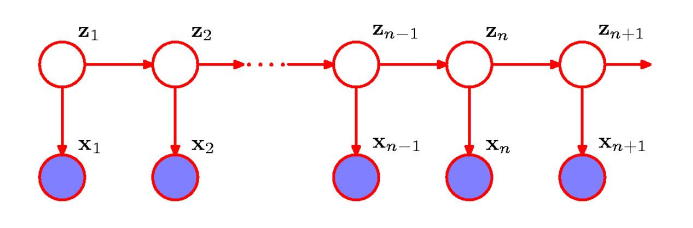
\includegraphics[width=\linewidth]{img/markov_diagram}
	\caption{Hidden Markov Model \label{hidden_diagram}}
\end{figure}

\begin{itemize}
	\item A hidden Markov Model is a collection of probabilities that tries to describe some sequential data 
  \begin{itemize}
  	\item The model depends on some discrete multinomial latent variable $\pmb z_i$ which is used to describe the probability of the corresponding observation $\pmb x_i$ 
    \item A 1 of $K$ coding scheme is used to describe the latent variables and the observations 
    \begin{itemize}
    	\item i.e. $z_{ik}$ means that the latent variable is in state $k$ at time $i$ 
    \end{itemize}
    \item The probability distribution of $\pmb z_i$ is allowed to depend on the state of the previous latent variable $\pmb z_{i-1}$ 
  \end{itemize}
  \item The conditional distribution is a $K$ dimensional binary variable and can therefore be described as a $K \times K$ table of numbers denoted $A$    
  \begin{itemize}
  	\item Its elements is known as \textbf{transition probabilities}
    \item They are given by $A_{jk} = p(z_{nk} = 1 \mid z_{n-1,j})$
    \item Since they are probabilities they must satisfy $0 \leq A_{jk} \leq 1$ with $\sum_k A_{jk} = 1$
    \item It has $K(K-1)$ independent variables 
    \item The conditional distribution can be explicitly written in the form
    \begin{equation*}
      p(\pmb z_n \mid \pmb z_{n-1, \pmb A}) = \prod_{k=1}^K \prod_{j=1}^K A_{jk}^{z_{n-1},jz_{nk}}
    \end{equation*}
  \end{itemize}
  \item The first latent variable $\pmb z_1$ is special since it does not have a parent node
  \begin{itemize}
    \item The distribution $p(\pmb z_1)$ is represented by a vector of probabilities $\pmb \pi$ where $\pmb \pi_k = p(z_{1k} = 1)$ so that 
    \begin{equation*}
      p(\pmb z_1 \mid \pmb \pi) = \prod_{k=1}^K \pi_k^{z_{1k}}
    \end{equation*}
where $\sum_k \pi_k = 1$ 
  \end{itemize} 
  \item The conditional distribution of the observed variables is given by $p(\pmb x_n \mid \pmb z_n, \phi)$, where $\phi$ is a set of parameters 
  \begin{itemize}
  	\item They are known as \textbf{emission probabilities}
    \item If the observed values are discrete e.g. $D$ symbols. Then the they can be described as a $K \times D$ table of probabilities    
    \begin{itemize}
    	\item Then an entry in the table is as follows $\phi_{jd} = p(x_{id} = 1 \mid z_{ij} = 1 )$ 
    \end{itemize}
    \item The emission probabilities can be written in the form  
    \begin{equation*}
      p(\pmb x_n \mid \pmb z_n, \phi) = \prod_{k=1}^K p(\pmb x_n \mid \phi_k)^{z_{nk}}
    \end{equation*}
  \end{itemize}
  \item The joint distribution over both latent and observed variables is given by
\begin{equation*}
  p(\pmb X, \pmb Z \mid \pmb \theta) = p(\pmb z_1 \mid \pmb \pi) \bigg [ \prod_{i=2}^n p(\pmb z_n \mid \pmb z_{n-1}, \pmb A) \bigg ] \prod_{m=1}^n p(\pmb x_m \mid \pmb z_m , \phi)
\end{equation*}
where $\pmb X = \{\pmb x_1, \dots, \pmb x_n\}, \pmb Z = \{\pmb z_1, \dots, \pmb z_n\}$, and $\pmb \theta = \{\pmb \pi, \pmb A, \phi \}$ denotes the set of parameters
  \begin{itemize}
  	\item One often computes the log probabilities since multiplying small numbers quickly become to small for a computer to represent 
  \end{itemize}
\end{itemize}

\subsection{Viterby decoding}
\begin{itemize}
	\item \textbf{Viterbi decoding:} $\pmb Z^*$ is the overall most likely explanation of $\pmb X$ :
\begin{equation*}
  \pmb Z^* = \arg\max_{\pmb{z}} p(\pmb X, \pmb Z \mid \pmb \Theta)
\end{equation*}
  \item To find the Viterby decoding of a given $X$ the following function is used   
\begin{equation*}
  \omega (\pmb z_n) \equiv \max_{\pmb z_1, \dots, \pmb z_{n-1}} p(\pmb x_1, \dots, \pmb x_n, \pmb z_1 \dots, \pmb z_n)
\end{equation*}
  \item Then the following holds for $p(\pmb X, \pmb Z^*)$ 
\begin{equation*}
	p(\pmb X, \pmb Z^*) = \max_{\pmb z_N} \omega (\pmb z_N)
\end{equation*}
  \item $\omega$ can be computed recursivly using the following which takes time $O(K^2N)$ and space $O(KN)$ using memorization
  \begin{itemize}
	  \item A table where $\omega[k][n] = \omega(\pmb z_n)$ if $\pmb z_n$ is state $k$
	  \item Basis: $\omega (\pmb z_1) = p(\pmb x_1, \pmb z_1) = p(\pmb z_1) p(\pmb x_1 \mid \pmb z_1)$
	  \item Recursion step: $\omega (\pmb z_n) = p(\pmb x_n \mid \pmb z_n) \max_{\pmb z_{z-1}} \omega (\pmb z_{n-1}) p(\pmb z_n \mid \pmb z_{n-1})$
  \end{itemize}
  \item To find $\pmb Z^*$ from the $\omega$ one can do backtracking on the table 
  \begin{itemize}
    \item $\pmb z^*_n$ is found by 
\begin{equation*}
  \pmb z^*_n = \arg \max_{\pmb z_n} \omega (\pmb z_n)
\end{equation*}
    \item All other $\pmb z^*_i$ is found by
\begin{equation*}
  z^*_i = \arg \max_{\pmb z_i} (p(\pmb x_{i+1} \mid \pmb z^*_{i+1}) \omega(\pmb z_i) p(\pmb z_{i+1}^* \mid \pmb z_i))
\end{equation*}
  	\item It takes $O(KN)$ time and space $O(KN)$ using $\omega$ 
  \end{itemize}
  \item To handle the very small floating numbers the log version of the probabilities is typically used instead where $\log(0)$ is defined to be $- \infty$ 
  \begin{itemize}
  	\item It also means that they should be added instead of multiplied
  \end{itemize}
\end{itemize}

\subsection{Posterior decoding}
\subsubsection{Normal version}
\begin{itemize}
	\item \textbf{Posterior decoding:} $\pmb z^*_n$ is the most likely state to be in the nth step
\begin{equation*}
  \pmb z^*_i = \arg \max_{\pmb z_i} p(\pmb z_i \mid \pmb x_1, \dots, \pmb x_n)
\end{equation*}
  \item The following two functions are defined  
\begin{align*}
  \alpha(\pmb z_i) &= p(\pmb x_1, \dots, \pmb x_i, \pmb z_i) \\
  \beta(\pmb z_i) &= p(\pmb x_{i+1}, \dots, \pmb x_n \mid \pmb z_n)
\end{align*}
  \item The $p(\pmb z_i \mid \pmb x_1, \dots, \pmb x_n)$ can be described in the following way given the two functions
\begin{align*}
  p(\pmb z_i \mid \pmb x_1, \dots, \pmb x_n) &= \frac{p(\pmb z_n, \pmb x_1, \dots, \pmb x_n)}{p(\pmb X)}\\
                                            &= \frac{p(\pmb x_1, \dots, \pmb x_i, \pmb z_i)  p(\pmb x_{i+1}, \dots, \pmb x_n \mid \pmb z_n)}{p(\pmb X)} \\
                                            &= \frac{\alpha(\pmb z_i) \beta(\pmb z_i)}{p(\pmb X)} 
\end{align*}
  thereby $\pmb z_i^* = \arg \max_{\pmb z_i} \alpha(\pmb z_i) \beta(\pmb z_i)/p(\pmb X)$ 
  \item Using $\alpha(\pmb z_i)$ and $\beta(\pmb z_i)$ one can get the likelihood of the observations as
\begin{equation*}
  p(\pmb X) = \sum_{\pmb z_i} \alpha (\pmb z_i) \beta(\pmb z_i) \quad p(\pmb X) = \sum_{\pmb z_n} \alpha (\pmb z_n)
\end{equation*}
	\item $\alpha$ can be computed using the following with takes time $O(K^2N)$ and space $O(KN)$ using memorization
  \begin{itemize}
	  \item A table where $\alpha[k][n] = \alpha(\pmb z_n)$ if $\pmb z_n$ is state $k$
	  \item Basis:  $\alpha(\pmb z_1) = p(\pmb x_1, \pmb z_1) = p(\pmb z_1)p(\pmb x_1 \mid \pmb z_1)$ 
	  \item Recursion step: $\alpha(\pmb z_i) = p(\pmb x_i \mid \pmb z_i) \sum_{\pmb z_{i-1}} \alpha (\pmb z_{i-1}) p(\pmb z_i \mid \pmb z_{i-1})$
  \end{itemize}
	\item $\beta$ can be computed using the following with takes time $O(K^2N)$ and space $O(KN)$ using memorization
  \begin{itemize}
	  \item A table where $\beta[k][n] = \beta(\pmb z_n)$ if $\pmb z_n$ is state $k$
	  \item Basis: $\beta(\pmb z_n) = 1 $ 
	  \item Recursion step: $\beta(\pmb z_i) = \sum_{i+1} \beta (\pmb z_{i+1} ) p(\pmb x_{i+1} \mid \pmb z_{i+1}) p(\pmb z_{i+1} \mid \pmb z_i)$
  \end{itemize}
  \item $\pmb z_i^*$ can then be found by first calculating the $\alpha$ and $\beta$ table and the taking arg max of the ith columns in the to tables multiplied divided by $p(\pmb X)$ 
\end{itemize}

\subsubsection{Number safe version}
\begin{itemize}
  \item To implement the forward algorithm without numeric problems $\hat \alpha (\pmb z_n)$ is used 
\begin{equation*}
	 \alpha (\pmb z_i) = \prod_{m=1}^i c_m \cdot \hat \alpha (\pmb z_i)
\end{equation*}
where $c_i = p (\pmb x_i \mid \pmb x_1, \dots, \pmb x_{i-1})$ 

  \item To compute the basis step the following formula is used
\begin{equation*}
  \hat \alpha (\pmb z_1) = \frac{\alpha(\pmb z_1)}{c_1}
\end{equation*}
where $c_1 = \sum_{k=1}^{K} \pi_k p(\pmb x_1 \mid \phi_k)$
  
 \item To compute the recursion step the following formula is used
\begin{equation*}
  \delta (\pmb z_{i}) = c_i \hat a (\pmb z_{i}) = p(\pmb x_i \mid \pmb z_i) \sum_{\pmb z_{i-1}} \hat \alpha (\pmb z_{i-1}) p(\pmb z_i \mid \pmb z_{i-1})
\end{equation*}
  \item The $c_i$ is computed an stored as
\begin{equation*}
	c_i = \sum_{k=1}^K \delta (z_{zk})
\end{equation*}
  \item Then compute and store $\hat \alpha(z_{ik}) = \delta(z_{ik})/c_i$ 

  \item To implement the backward algorithm without numeric problems $\hat \beta (\pmb z_i)$ is used 
\begin{equation*}
  \hat \beta = {\beta(\pmb z_b)}{\prod_{m=i+1}^n c_m}
\end{equation*}
  \item The basis step is $\hat \beta (\pmb z_n) = 1$ as the unscaled version
  \item The recursion step $i$ is to compute the following $K$ values $\epsilon(z_{i1}), \dots, \epsilon(z_{iK})$ 
\begin{equation*}
  \epsilon (\pmb z_i) = c_{i+1} \hat \beta(\pmb z_i) = \sum_{z_{i+1}} \hat \beta (\pmb z_{i+1}) p(\pmb x_{i+1} \mid \pmb z_{i+1}) p(\pmb z_{i+1} \mid \pmb z_i)
\end{equation*}
  \item Using the $c_{i+1}$ computed during forward recursion compute and store $\hat \beta (z_{ik}) = \epsilon (z_{ik}) / c_{i+1}$ 

  \item Using the scaled versions $\hat \alpha$ and $\hat \beta$ the following holds
\begin{align*}
  p(\pmb z_i \mid \pmb x_1, \dots, \pmb x_i) &= \frac{\alpha (\pmb z_i) \beta (\pmb z_i)}{p(\pmb X)}\\
                                            &= \frac{\hat \alpha (\pmb z_i) (\prod_{m=1}^i c_m) \hat \beta (\pmb z_i)(\prod_{m=i+1}^n c_m)}{(\sum_{m=1}^nc_m)} \\
                                            &= \hat \alpha (\pmb z_n) \hat \beta (\pmb z_n)
\end{align*}

  \item Then the posterior decoding $\pmb z_n^*$ for a given $n$ becomes
\begin{equation*}
  \pmb z_n^* = \arg \max_{\pmb z_n} \hat \alpha (\pmb z_n)  \hat \beta (\pmb z_n)
\end{equation*}
\end{itemize}
  
\newpage

\section{Hidden Markov Models  Training}
\subsection{Disposition}
\begin{enumerate}
	\item Definition
  \begin{itemize}
  	\item Latent variables and observations
    \item Transitions probabilities
    \item Start probabilities 
    \item Emission probabilities
    \item Joint distribution
  \end{itemize}
  \item Training by counting
  \begin{itemize}
    \item Uses observation and concrete latent variable
    \item Definition of parameters
    \item Psuedocount
  \end{itemize}
  \item Viterby training
  \begin{itemize}
  	\item Only based on observation
    \item Algorithm
    \item Does not maximize maximum likelihood 
  \end{itemize}
  \item EM
  \begin{itemize}
  	\item Definition of $Q$ 
    \item Why maximizing $Q$ improves MLE
    \item Definition of maximizing expression 
    \item Calculation of expectation
    \item New Algorithm
    \item EM Algorithm
    \item Scaled version
  \end{itemize}
\end{enumerate}
\newpage

\subsection{Definition}
\begin{figure}[h]
	\centering
	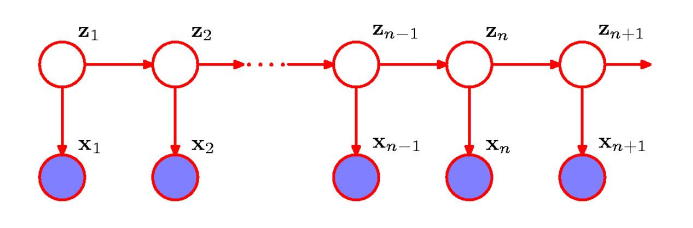
\includegraphics[width=\linewidth]{img/markov_diagram}
	\caption{Hidden Markov Model \label{hidden_diagram2}}
\end{figure}

\begin{itemize}
	\item A hidden Markov Model is a collection of probabilities that tries to describe some sequential data 
  \begin{itemize}
  	\item The model depends on some discrete multinomial latent variable $\pmb z_i$ which is used to describe the probability of the corresponding observation $\pmb x_i$ 
    \item A 1 of $K$ coding scheme is used to describe the latent variables and the observations 
    \begin{itemize}
    	\item i.e. $z_{ik}$ means that the latent variable is in state $k$ at time $i$ 
    \end{itemize}
    \item The probability distribution of $\pmb z_i$ is allowed to depend on the state of the previous latent variable $\pmb z_{i-1}$ 
  \end{itemize}
  \item The conditional distribution is a $K$ dimensional binary variable and can therefore be described as a $K \times K$ table of numbers denoted $A$    
  \begin{itemize}
  	\item Its elements is known as \textbf{transition probabilities}
    \item They are given by $A_{jk} = p(z_{nk} = 1 \mid z_{n-1,j})$
    \item Since they are probabilities they must satisfy $0 \leq A_{jk} \leq 1$ with $\sum_k A_{jk} = 1$
    \item It has $K(K-1)$ independent variables 
    \item The conditional distribution can be explicitly written in the form
    \begin{equation*}
      p(\pmb z_n \mid \pmb z_{n-1, \pmb A}) = \prod_{k=1}^K \prod_{j=1}^K A_{jk}^{z_{n-1},jz_{nk}}
    \end{equation*}
  \end{itemize}
  \item The first latent variable $\pmb z_1$ is special since it does not have a parent node
  \begin{itemize}
    \item The distribution $p(\pmb z_1)$ is represented by a vector of probabilities $\pmb \pi$ where $\pmb \pi_k = p(z_{1k} = 1)$ so that 
    \begin{equation*}
      p(\pmb z_1 \mid \pmb \pi) = \prod_{k=1}^K \pi_k^{z_{1k}}
    \end{equation*}
where $\sum_k \pi_k = 1$ 
  \end{itemize} 
  \item The conditional distribution of the observed variables is given by $p(\pmb x_n \mid \pmb z_n, \phi)$, where $\phi$ is a set of parameters 
  \begin{itemize}
  	\item They are known as \textbf{emission probabilities}
    \item If the observed values are discrete e.g. $D$ symbols. Then the they can be described as a $K \times D$ table of probabilities    
    \begin{itemize}
    	\item Then an entry in the table is as follows $\phi_{jd} = p(x_{id} = 1 \mid z_{ij} = 1 )$ 
    \end{itemize}
    \item The emission probabilities can be written in the form  
    \begin{equation*}
      p(\pmb x_n \mid \pmb z_n, \phi) = \prod_{k=1}^K p(\pmb x_n \mid \phi_k)^{z_{nk}}
    \end{equation*}
  \end{itemize}
  \item The joint distribution over both latent and observed variables is given by
\begin{equation*}
  p(\pmb X, \pmb Z \mid \pmb \Theta) = p(\pmb z_1 \mid \pmb \pi) \bigg [ \prod_{i=2}^n p(\pmb z_n \mid \pmb z_{n-1}, \pmb A) \bigg ] \prod_{m=1}^n p(\pmb x_m \mid \pmb z_m , \phi)
\end{equation*}
where $\pmb X = \{\pmb x_1, \dots, \pmb x_n\}, \pmb Z = \{\pmb z_1, \dots, \pmb z_n\}$, and $\pmb \Theta = \{\pmb \pi, \pmb A, \phi \}$ denotes the set of parameters
  \begin{itemize}
  	\item One often computes the log probabilities since multiplying small numbers quickly become to small for a computer to represent 
  \end{itemize}
\end{itemize}
  
\subsection{Training by counting}
\begin{itemize}
	\item Training by counting can be used if sequences of observations $\pmb X = \{\pmb x_1, \dots, \pmb x_n\}$ and the corresponding latent states $\pmb Z = \{\pmb z_1, \dots, \pmb z_n\}$ is known
  \item It counts how many times a transition of emission is observed 
  \item The following equations is used to define the probabilities
  \begin{equation*}
    A_{jk} = \frac{\sum_{i=2}^n z_{i-1,j}z_{ik}}{\sum_{l=1}^k\sum_{i=2}^n z_{i-1,j}z_{il}}  \quad
    \pi_k = \frac{z_{1k}}{\sum_{j=1}^Kz_{1j}} \quad
    \phi_{jk}=\frac{\sum_{i=1}^n z_{ik}x_{ij}}{\sum_{i=1}^n z_{ik}} 
  \end{equation*}
  \item It yields the maximum likelihood estimate $\pmb \Theta^*$ of $p(\pmb X, \pmb Z \mid \pmb \Theta)$ which is what we want
  \item There is a problem with this model, if a transition from a state $j$ to a state $k$ is not observed, then probability $A_{jk}$ is set to $0$  
  \begin{itemize}
  	\item A practical solution is to assume that every transmission and emission is seen once   
    \item It is called psuedocount
  \end{itemize}
\end{itemize} 

\subsection{Viterby training}
\begin{itemize}
	\item Viterby training can be used if only sequences of observations $\pmb X = \{\pmb x_1, \dots, \pmb x_n\}$ known and the corresponding latent states $\pmb Z = \{\pmb z_1, \dots, \pmb z_n\}$ is unknown  
  \item Direct maximization of the likelihood is hard
  \begin{equation*}
    p(\pmb X \mid \Theta) = \sum_{\pmb Z} p(\pmb X, \pmb Z \mid \Theta)
  \end{equation*}

  \item Viterbi training is done as follows  
  \begin{enumerate}
  	\item Decide on some initial parameter $\Theta ^0$  
    \item Find the most likely sequence of states $\pmb Z^*$ explaining $\pmb X$ using the Viterby Algorithm and the current parameters $\pmb \Theta ^i$  
    \item Update parameters to $\pmb \Theta^{i+1}$ by counting with psuedocount according to $(\pmb X, \pmb Z^*)$ 
    \item Repead 2-3 until $P(\pmb X, \pmb Z^* \mid \pmb \Theta^i)$ is satisfactory or the Viterby sequence of states does not change
  \end{enumerate}
  \item It finds a local maximum of
  \begin{equation*}
    \mathsf{VIT}_{\pmb X}(\pmb \Theta) = \max_{\pmb Z} p(\pmb X, \pmb Z \mid \pmb \Theta)
  \end{equation*}
  It works okay even though it is not a maximum likelihood
\end{itemize}  

\subsection{EM}
\begin{itemize}
	\item EM can also be used if only sequences of observations $\pmb X = \{\pmb x_1, \dots, \pmb x_n\}$ is known and the corresponding latent states $\pmb Z = \{\pmb z_1, \dots, \pmb z_n\}$ is unknown  
  \item The following formula is defined
  \begin{equation*}
    Q(\pmb \Theta, \pmb \Theta^\text{old}) = \sum_{\pmb Z} p(\pmb Z \mid \pmb X, \Theta^\text{old}) \log p(\pmb X, \pmb Z \mid \pmb \Theta)
  \end{equation*}
  \item The following fact is used 
  \begin{equation*}
    p(\pmb X \mid \pmb \Theta) = \frac{p(\pmb X, \pmb Z \mid \pmb \Theta)}{p(\pmb Z \mid \pmb X, \pmb \Theta)}
  \end{equation*}
  \item We derive another expression for $\log p(\pmb X \mid \pmb \Theta)$ 
  \begin{align*}
     \log p(\pmb X \mid \pmb \Theta) &= \sum_{\pmb Z} p(\pmb Z \mid \pmb X, \pmb \Theta^\text{old}) \log p(\pmb X \mid \pmb \Theta) \text{  (Sums to one)} \\
                                     &= \sum_{\pmb Z} p(\pmb Z \mid \pmb X, \pmb \Theta^\text{old})( \log p(\pmb X , \pmb Z \mid \pmb \Theta) - \log p(\pmb Z \mid \pmb X, \pmb \Theta)) \\
                                     &= \sum_{\pmb Z} p(\pmb Z \mid \pmb X, \pmb \Theta^\text{old}) \log p(\pmb X , \pmb Z \mid \pmb \Theta) - \sum_{\pmb Z} p(\pmb Z \mid \pmb X, \pmb \Theta^\text{old}) \log p(\pmb Z \mid \pmb X, \pmb \Theta) \\
                                     &= Q(\pmb \Theta, \pmb \Theta^\text{old})- \sum_{\pmb Z} p(\pmb Z \mid \pmb X, \pmb \Theta^\text{old}) \log p(\pmb Z \mid \pmb X, \pmb \Theta) 
  \end{align*}
  \item Given a valid set of parameters $\pmb \theta^\text{old}$, we want to estimate a set of valid parameters $\pmb \Theta$ that gives a better likelihood. We have
  \begin{align*}
    \log p(\pmb X \mid \pmb \Theta) &= Q(\pmb \Theta, \pmb \Theta^\text{old})- \sum_{\pmb Z} p(\pmb Z \mid \pmb X, \pmb \Theta^\text{old}) \log p(\pmb Z \mid \pmb X, \pmb \Theta) \\
    \log p(\pmb X \mid \pmb \Theta^{\text{old}}) &= Q(\pmb \Theta^\text{old}, \pmb \Theta^\text{old})- \sum_{\pmb Z} p(\pmb Z \mid \pmb X, \pmb \Theta^\text{old}) \log p(\pmb Z \mid \pmb X, \pmb \Theta^\text{old}) 
  \end{align*}
  \item This means that the increase can be written as 
  \begin{align*}
    \log p(\pmb X \mid \pmb \Theta) - &\log p(\pmb X \mid \pmb \Theta^\text{old}) = \\ & Q(\pmb \Theta, \pmb \Theta^\text{old}) - Q(\pmb \Theta, \pmb \Theta^\text{old}) + \sum_{\pmb Z} p(\pmb Z \mid \pmb X, \Theta^\text{ikd})\log \frac{p(\pmb Z \mid \pmb X , \Theta ^\text{old})}{p(\pmb Z \mid \pmb X, \pmb \Theta)}
  \end{align*}
  \item Since the last part of the equation is the relative entropy of $p(\pmb Z \mid \pmb X, \pmb \Theta^\text{old})$ relative to $p(\pmb Z \mid X, \pmb \Theta)$ and is therefore $\geq 0$ the following must hold
 \begin{equation*}
    \log p(\pmb X \mid \pmb \Theta) - \log p(\pmb X \mid \pmb \Theta^\text{old}) \geq Q(\pmb \Theta, \pmb \Theta^\text{old}) - Q(\pmb \Theta^\text{old}, \pmb \Theta^\text{old}) 
 \end{equation*}
  \item This means that by maximizing the expectation $Q(\pmb \Theta, \pmb \Theta^\text{old})$ with respect to $\pmb \Theta$ we increase the likelihood
  \item Taking the expectation (under $\pmb \Theta ^\text{old}$) over all $\pmb Z$'s yields $Q(\pmb \Theta, \pmb \Theta^\text{old})$ 
  \begin{equation*}
    Q(\pmb \Theta, \pmb \Theta^\text{old}) = \sum_{k=1}^KE(z_{1k}) \log \theta_k + \sum_{i=2}^n \sum_{j=1}^K\sum_{k=1}^K z_{i.1,j}z_{ik} \log A_{jk} + \sum_{i=1}^n\sum_{k=1}^K E(z_{nk}) \log p(\pmb x_n \mid \phi_k)
  \end{equation*}
  \item The following expressions is defined 
  \begin{align*}
              \gamma(\pmb z_i) &= p(\pmb z_i \mid \pmb X, \pmb \Theta^\text{old}) \\
    \xi(\pmb z_{i-1}, \pmb z_n) &= p(\pmb z_{i-1}, \pmb z_i \mid \pmb X, \pmb \Theta^\text{old})
  \end{align*}
  \item Since the expectation of a binary variable $z$ is just $p(z=1)$, the following then holds 
  \begin{align*}
                    E(z_{ik}) = \gamma(z_{ik}) &= \sum_{\pmb Z} \gamma (\pmb z_i) z_{nk} \\
    E(z_{i-1,j}, z_{nk}) = \xi(z_{i-1,j}, z_{ij}) &= \sum_{\pmb Z} \xi(\pmb z_{n-1}, \pmb z_n) z_{n-1,j} z_{nk}
  \end{align*}
  \item If we assumed discrete observables $\pmb x_i$, then maximizing the equation yields 
  \begin{equation*}
    A_{jk} = \frac{\sum_{i=2}^n \xi(z_{i-1,j},z_{ik})}{\sum_{l=1}^k\sum_{i=2}^n \xi(z_{i-1,j},z_{il})}  \quad
    \pi_k = \frac{\gamma(z_{1k})}{\sum_{j=1}^K\gamma(z_{1j})} \quad
    \phi_{jk}=\frac{\sum_{i=1}^n \gamma(z_{ik})x_{ij}}{\sum_{i=1}^n \gamma(z_{ik})} 
  \end{equation*}
  \item $\gamma(\pmb z_i)$ and $\xi(\pmb z_{n-1}, \pmb z_n)$ can be computed by
  \begin{align*}
             \gamma(\pmb z_i) &= \frac{\alpha(\pmb z_i) \beta(\pmb z_i)}{p(\pmb X)} \\
   \xi(\pmb z_{i-1}, \pmb z_i) &= \frac{\alpha(z_{i-1}) \beta(\pmb z_i) p(\pmb z_n \mid \pmb z_{n-1}) p(\pmb x_n \mid \pmb z_n)}{p(\pmb X)}
  \end{align*}
  which can be computed efficiently using the forward- and backward-algorithm
  \item The EM algorithm is as follows
  \begin{enumerate}
  	\item \textbf{Init:} pick suitable parameters
    \begin{itemize}
    	\item Transition and emission probabilities
      \item A parameters should not be initialized to zero as it remains zero 
    \end{itemize}
    \item \textbf{E-Step:} Run the forward and backward-algorithms with the current choice of parameters
    \item \textbf{Stop?:} Compute the likelihood $p(\pmb X \mid \pmb \Theta)$ if sufficient or other stopping criteria is meet stop
    \item \textbf{M-Step:} Compute the new parameters using the values stored by the forward- and backward-algorithms
  \end{enumerate}
  \item The running time of the algorithm is $O(K^2n + KK + K^2NK + KDN)$ where $D$ is the number of observables and it can be improved to $O(K^2N + KDN)$ by using memorization in 3.  
  \item To use the number safe scaled values in the EM the following equations can be used
  \begin{align*}
             \gamma(\pmb z_n) &= \hat \alpha (\pmb z_n) \hat \beta(\pmb z_n) \\
   \xi(\pmb z_{i-1}, \pmb z_i) &= \hat \alpha(z_{i-1}) \hat \beta(\pmb z_i) p(\pmb z_n \mid \pmb z_{n-1}) p(\pmb x_n \mid \pmb z_n)/c_n
  \end{align*}
\end{itemize}

\newpage

\section{Dimensionality reduction and representative based clustering}
\subsection{Disposition}
\begin{enumerate}
	\item Principal Component Analysis
  \begin{itemize}
  	\item Dimensionality reduction in general
    \item Task of PCA
    \item Covariance matrix
    \item Diagonalizing and eigenvalues
    \item Mapping vectors
    \item Reconstruction error
  \end{itemize}
  \item K-means
  \begin{itemize}
  	\item Representative based clustering
    \item Centroid
    \item Scoring function
    \item Llouds algorithm
  \end{itemize}
  \item Expectation-Maximization 
  \begin{itemize}
  	\item Soft assignment clustering
    \item Distribution
    \item Model parameters
    \item Algorithm
  \end{itemize}
\end{enumerate}
\newpage

\subsection{Principal Component Analysis}
\begin{itemize}
  \item \textbf{Dimensionality reduction} is done linearly
  \begin{itemize}
  	\item It should be possible to construct the original data point from the optimal subspace as well as possible  
	  \item The mean squared distance between original and reconstructed data points is the \textbf{reconstruction error}
    \item One typically removes the mean value from the data before doing dimensionality reduction
    \begin{itemize}
    	\item Zero mean data is assumed throughout
    \end{itemize}
  \end{itemize}
	\item The task of \textbf{principal component analysis} is to reduce the dimensionality of some high-dimensional data point
  \begin{itemize}
  	\item It is done by projecting them onto a lower dimensional space in a way that the reconstruction error minimal
    \item Minimizing the construction error is equivalent to maximizing the variance of the projected data
  \end{itemize}
  \item The \textbf{convariance matrix} assumes zero mean data and has the componenets $C_{ij} := \langle x_ix_j \rangle$  
  \begin{itemize}
  	\item The data points are written as $\pmb x = (x_1, x_2)^T$
    \item The variance of the first and second component can be written as $C_{11} := \langle x_1x_1 \rangle$ and $C_{22} := \langle x_2x_2 \rangle$
    \begin{itemize}
    	\item The angle brackes indicate averaging over all data points
      \item If $C_{11}$ is large compared to $C_{22}$ the direction of maximal variance is close to $(1,0)^T$
      \item If $C_{11}$ is small the direction of maximal variance is close to $(0,1)^T$
    \end{itemize}
    \item If $C_{11}$ and $C_{22}$ are similar the covariance between the two components $C_{12} := \langle x_1x_1 \rangle$ can give additional information
    \begin{itemize}
      \item A large positive value indicate a strong correlation and then $(1,1)^T$ should be used
      \item A negative value would indicate anti-correlation and then $(-1,1)^T$ should be used
      \item A small value would indicate no correlation, i.e. no prominent direction of maximal variance
    \end{itemize}

    \item The components obey the relation: $C_{ij} \leq C_{ii} C_{jj}$
  	\item Scaling the data by a factor $\alpha$ scales the matrix by a factor $\alpha^2$ 
  \end{itemize}
  \item If the covariance matrix is diagonal the maximal variance is the axis belong to the largest value of the covariance matrix 
  \begin{itemize}
  	\item A non-diagonal covariance matrix can be made diagonal by rotating the coordinate system accordingly
    \item Diagonalizing a matrix can be done by solving the corresponding eigenvalue equation
    \item The eigenvectors of the covariance matrix point to the directions of maximal and minimal variance
    \item The eigenvalues are equal to the variances along these directions
  	\item Projecting the data onto the eigenvectors with largest eigenvalues is therefore the optimal linear dimensionality reduction. 
  \end{itemize}
  \item The covariance matrix can be written as follows in vector notation
  \begin{equation*}
    C_x := \langle \pmb x \pmb x^T \rangle = \frac1n \sum_{i=1}^n \pmb x_i \pmb x_i^T
  \end{equation*}
\end{itemize}

\subsubsection{Mapping Vectors}
\begin{itemize}
	\item If we are given $P$ $I$-dimensional vectors $\pmb v_p$ that map into the low-dimensional coordinate system, where $P < I$ the vectors can be arranged into a matrix
  \begin{equation*}
    V := (\pmb v_1, \pmb v_2, \dots, \pmb v_P)
  \end{equation*}
  \begin{itemize}
  	\item The vectors $\pmb v_1$ and $\pmb v_2$ should also be pairwise orthogonormal
  \end{itemize}
  \item The matrix can be used to map the data points $\pmb x$ into the subspace spanned by the vectors $v_p$ by using the following formula
  \begin{equation*}
    \pmb y := \pmb V^T \pmb x
  \end{equation*}
  \item The matrix can also be used to map the point back to the old space by using the following equation
  \begin{equation*}
    \pmb x_{||} := \pmb V \pmb y = \pmb V \pmb V^T \pmb x
  \end{equation*}
  $\pmb y$ and $\pmb x_{||}$ are equivalent representations
  \begin{itemize}
    \item The contain the same information just in different coordinate systems 
  \end{itemize}
\end{itemize}

\subsubsection{Reconstruction Error}
\begin{itemize}
  \item The reconstruction error $E$ is defined as the mean square sum over the distances between the orginal data points $\pmb x$ and the projected ones $\pmb x_{||}$
  \item If we define the orthogonal vectors
\begin{equation*}
  \pmb x_\bot = \pmb x - \pmb x_{||}
\end{equation*}
  The following result can be found 
\begin{equation*}
  E = \langle \pmb x_{\bot}^T \pmb x_{\bot} \rangle - \langle \pmb y^T \pmb y \rangle 
\end{equation*}
\item The reconstruction error equals the difference between the variance of the data minus the variance of the projected data.
\end{itemize}

\newpage
\subsection{K-means}
\begin{framed}
\begin{center}  
  \textbf{Lloyds Algorithm}
\end{center}
\begin{lstlisting}[mathescape=true, keywordstyle=\ttfamily]
Lloyds($\pmb D, k, \epsilon $):
  $t=0$  
  Randomly initialize $k$ centroids: $\pmb \mu_1^t,\pmb \mu_2^t, \dots,\pmb \mu_k^t \in \R^d$
  repeat 
    $t \leftarrow t+1$ 
    $C_j \leftarrow \emptyset$ for all $j= 1, \dots, k$ 
    // Cluster Assignment Step
    foreach $\pmb x_j \in \mathbf D$ do
      $j^* \leftarrow \arg \min \big\{|| \pmb x_j - \pmb \mu_i^{t-1}||^2\big\}$ 
      $C_{j^*} \leftarrow C_{j^*} \cup \{\pmb x_j\}$
    // Centroid update step
    foreach $i=1 \text{ to } k$ do
      $\pmb \mu_i^t \leftarrow \frac1{|C_i|} \sum_{\pmb x_j \in C_i} \pmb x_j$
  until $\sum_{i=1}^k ||\pmb \mu_i^t- \pmb \mu_i^{t-1}||^2 \leq \epsilon$
\end{lstlisting}
\end{framed}
\begin{itemize}
	\item \textbf{K-means} is a type of \textbf{representative-based clustering}
  \begin{itemize}
  	\item The goal of it given a data set $D = (\pmb x_1, \dots, \pmb x_n)$ and a number of clusters $k$ is to divide a given data set into $k$ clusters 
	  \item This is called a \textbf{clustering}
  	\item It is denoted as $\mathcal C = \{C_1, C_2, \dots, C_k\}$
    \item For each cluster $C_i$ there exists a representative point that summerizes the cluster 
  \end{itemize}
  \item In K-means the representative point that summerizes the cluster is the mean (centroid) $\pmb \mu_i$ og all points in the clusters i.e.
\begin{equation*}
  \pmb \mu_i = \frac1{n_i} \sum _{x_j \in C_i} \pmb x_j
\end{equation*}
where $n_i = |C_i|$
  \item Given a clustering $\mathcal C = \{C_1, C_2, \dots, C_k\}$ a the \textbf{sum of squared error} scoring function is defined as
  \begin{equation*}
    SSE(\mathcal C) = \sum_{i=1}^k \sum_{\pmb x_j \in C_i} ||\pmb x_j - \pmb \mu_i ||^2
  \end{equation*}
  The goal is to finding the clustering that minimizes the SSE score 
  \begin{equation*}
    C^* = \arg \min_{\mathcal C} \{SSE(\mathcal C)\}
  \end{equation*}
  \item Lloyds algortihm uses a greedy iterative approach to find the clustering that minimizes the score
  \begin{itemize}
  	\item It can converge to a local optima instead of a global optimal clustering  
    \item Since it is randomly initialized it is typically runned a couple of times and the one with the lowest score is chosen    
  	\item It generates convex shaped clusters
  	\item The total time for K-means is given as $O(tnkd)$
    \begin{itemize}
      \item Where $t$ is the number of iterations
      \item $d$ is the number of dimensions 
    \end{itemize}
  \end{itemize}
\end{itemize}

\subsection{Expectation-Maximization Clustering}
\begin{itemize}
	\item Expectation Maximization is a \textbf{soft assignment clustering} where each point has a probability of belonging to each cluster
  \item It is assumed that each cluster $C_i$ is characterized by the multivariate normal distribution i.e.
  \begin{equation*}
    f_i(\pmb x) = f(\pmb x \mid \pmb \mu_i, \pmb \Sigma_i) = \frac1{(2\pi)^{\frac d2}|\pmb \Sigma_i|^{\frac12}} \exp \bigg\{-\frac{(\pmb x- \pmb \mu_i)^T \pmb \Sigma_i^{-1}(\pmb x-\pmb  \mu_i)}2\bigg\}
  \end{equation*}
  where the clusters mean $\pmb \mu_i \in \mathbb R^d$ and the covariance matrix $\mathbf \Sigma \in \mathbb R^{d \times d}$ are unknown parameters
	\item $f_i(\pmb x)$ is the probability density at $\pmb x$ attributable to cluster $C_i$
  \begin{itemize}
	  \item It is assumed that the probability density function of $\mathbf X$ is given as a Gaussian mixture model over all the $k$ cluster normals, defined as 
  \begin{equation*}
    f(\pmb x) = \sum_{i=1}^k f_i(\pmb x_j) P(C_i)
  \end{equation*}
    The prior probabilities $P(C_i)$ are called the \textbf{mixture parameters} and must satisfy the condition 
  \begin{equation*}
    \sum_{i=1}^kP(C_i) = 1
  \end{equation*}
  \end{itemize}
  \item The model parameters can be written compactly as 
  \begin{equation*}
    \pmb \theta = \bigg\{\pmb \mu_1, \Sigma_1, P(C_1), \dots, \pmb \mu_k, \Sigma_k, P(C_k)\bigg\} 
  \end{equation*}
  \item The goal is to maximize the probability of the data i.e. maximizing $P(\pmb D \mid \pmb \theta)$ 
  \begin{itemize}
  	\item The log-likelihood version is used
    \item Since maximizing the log-likelihood over $\mathbf \theta$ directly is hard expectation maximization is used instead
  \end{itemize}
\end{itemize}
\newpage

\begin{framed}  
\begin{center}  
  \textbf{Expectation Maximization Algorithm} 
\end{center}
\begin{lstlisting}[mathescape=true, keywordstyle=\ttfamily]
EXPECTATION-MAXIMIZATION($\pmb D, k, \epsilon$):
  $t \leftarrow 0$ 
  // Initialization
  Randomly initialize $\pmb \mu_1^t, \dots, \pmb \mu_k^t$ 
  $\Sigma_i^t \leftarrow \mathbf I, \forall i = 1, \dots,k$ 
  $P^t(C_i) \leftarrow \frac1k,\forall i = 1, \dots,k$
  repeat
    $t \leftarrow t+1$
    // Expectation Step
    for $i=1, \dots, k$ and $k=1, \dots,n$ do i
      $w_{ij} \leftarrow  \frac{f_i(\pmb x_j) \cdot P(C_i)}{\sum_{a=1}^kf_a(\pmb x_j) \cdot P(C_a)}$ //posterior probability $P^t(C_i \mid \pmb x_j)$ 
    // Maximization Step
    $\pmb \mu_i = \frac{\sum_{j=1}^nw_{ij} \cdot \pmb x_j}{\sum_{j=1}^nw_{ij}}$ // re-estimate mean
    $\mathbf \Sigma_i^t \leftarrow \frac{\sum_{j=1}^nw_{ij}(\pmb x_j- \pmb \mu_i)(\pmb x_j-\pmb u_i)^T}{\sum_{j=1}^nw_{ij}}$ // re-estimate covariance matrix
    $P^t(c_i) \leftarrow \frac{\sum_{j=1}^n w_{ij}}{n}$ // re-estimate priors 
  until $\sum_{k=1}^k || \pmb \mu_i^t - \pmb \mu_i^{t-1}||^2 \leq \epsilon$ 
\end{lstlisting}
\end{framed}
\newpage 

\section{Density-based and hierarchical clustering}
\subsection{Disposition}
\begin{enumerate}
	\item Density-Based clutering 
  \begin{itemize}
    \item Definition
  	\item $\epsilon$-neighborhood
    \item Core point
    \item Border point
    \item Noise
    \item Density reachable
    \item Density-based cluster
  \end{itemize}
  \item DBSCAN
  \begin{itemize}
  	\item Algortihm
    \item Limitation
    \item Time complexity
  \end{itemize}
  \item DENCLUE
  \begin{itemize}
  	\item Density estimation and clustering
    \item Function
    \item Kernels
    \item Gradient Ascent and Direct update rule
    \item Algorithm
  \end{itemize}
\end{enumerate}
\newpage

\subsection{Density-based clustering}
\begin{itemize}
	\item \textbf{Density-based clustering} uses the local density of points to determine the clusters
  \item A ball of radius $\epsilon$ is defined around the point $\pmb x \in \R^d$ called the $\epsilon$-neighborhood as follows
  \begin{equation*}
    N_\epsilon (\pmb x) = B_d(\pmb x, \epsilon) = \{ \pmb y \mid \delta(\pmb x, \pmb y) \leq \epsilon \}
  \end{equation*}
  The distance measure is usually assumed to be the Euclidean distance $\delta(\pmb x, \pmb y) = ||\pmb x- \pmb y ||_2$
  \item A \textbf{core point} is a point with at least $minpts$ points in its $\epsilon$-neighborhood 
  \item A \textbf{border point} is a point that is not a core point but belongs to the $\epsilon$-neighborhood of some core point  
  \item An \textbf{outlier} or \textbf{noise point} is a point that is neither a border or core point 
  \item A point $\pmb x \in \R^d$ is \textbf{directly density reachable} from another point $\pmb y \in \R^d$ if $\pmb x \in N_\epsilon(\pmb y)$ and $\pmb y$ is a core point
	\item $\pmb x$ is \textbf{density reachable} if their exists a chain of point $\pmb x_0, \pmb x_1, \dots, \pmb x_l$ such that $\pmb x = \pmb x_0$ and $\pmb y = \pmb x_i$ and $\pmb x_i$ is directly density reachable from $\pmb x_{i-1}$ for all $i=1, \dots,l$
  \begin{itemize}
  	\item It is an asymmetric relationship
  \end{itemize}
	\item A \textbf{density-based cluster} is defined as the maximal set of density connected points 
\end{itemize}

\subsection{DBSCAN}
\begin{framed}  
\begin{center}  
  \textbf{DBSCAN Algorithm}  
\end{center}
\begin{lstlisting}[mathescape=true, keywordstyle=\ttfamily]
DBSCAN($\mathbf D, \epsilon, minpts $):
  Core $\leftarrow \emptyset$ 
  foreach $\pmb x_i \in \mathbf D$ do // Find the core points
    Compute $N_\epsilon(\pmb x_i)$ 
    $id(\pmb x_i) \leftarrow \emptyset$ // cluster id for $\pmb x_i$ 
    if $N_\epsilon (\pmb x_i) \geq minpts$ then $Core \leftarrow Core \cup \{\pmb x_i\}$ 
  $k \leftarrow 0$ // cluster id 
  foreach $\pmb x_i \in Core$, such that $id(\pmb x_i) = \emptyset$ do  
    $k \leftarrow k+1$ 
    $id(\pmb x_i) \leftarrow k$ // assign $\pmb x_i$ to cluster id $k$ 
    DENSITYCONNECTED($\pmb x_i,k$)
  $\mathcal C \leftarrow \{C_i\}_{i=1}^k$, where $C_i \leftarrow \{\pmb x \in \mathbf{D} \mid id(\pmb x) = i\}$ 
  $Noise \leftarrow \{\pmb x \in \mathbf D \mid id(\pmb x) = \emptyset\}$
  $Border \leftarrow \mathbf D \backslash \{Core \cup Noise\}$ 
  return $\mathcal C, Core, Border, Noise$ 

DENSITYCONNECTED($\pmb x, k$):
  foreach $\pmb y \in N_\epsilon(\pmb x)$ such that $id(\pmb y) = \emptyset$ do
    $id(\pmb y) \leftarrow k$ // assign $\pmb y$ to cluster id $k$ 
    if $\pmb y \in Core$ then DENSITYCONNECTED($\pmb y,k$)  
\end{lstlisting}
\end{framed}
\begin{itemize}
  \item DBSCAN computes the $\epsilon$ neighborhood $N_\epsilon(\pmb x_i)$ for each point $\pmb x_i$ in the data set $\mathbf D$ and checks if it is a core point
  \begin{itemize}
  	\item It sets the cluster id $id(\pmb x_i) = \emptyset$ for all points, which indicates that they has not been assigned to any cluster
  	\item Starting from each unassigned core point, the method recursively finds all its density connected points, which are assigned to the same cluster
	  \item Some border point may be reachable from core points in more than one cluster
    \begin{itemize}
    	\item They may be assigned to one of the cluster or all of them - if overlapping clusters are allowed 
    \end{itemize}
  \end{itemize}
  \item A limitation of DBSCAN is that is sensitive to the choice of $\epsilon$
  \begin{itemize}
	  \item If $\epsilon$ is too small, sparser clusters will be categorized as noise
  	\item If $\epsilon$ is too large denser clusters may be merge together
	  \item If there are clusters with different local densities a single $\epsilon$ value may not suffice 
  \end{itemize}
  \item If the dimensionality is not too high the DBSCAN takes $O(n \cdot \log(n))$ time
  \begin{itemize}
	  \item Worst case it takes $O(n^2)$ time
  \end{itemize}
\end{itemize}

\subsection{DENCLUE}
\begin{itemize}
  \item There is a close connection between density-based clustering and density estimation
  \begin{itemize}
	  \item The goal of density estimation is to find an unknown probability density function by finding the dense regions of points which in turn can be used for clustering
  	\item It tries to directly infer the underlying probability density at each point in the dataset 
  \end{itemize}
  \item To estimate the probability density at a $d$ dimensional points $\pmb x = (x_1, x_2, \dots, x_d)^T$ a $d$ dimensional window is defined
  \begin{itemize}
  	\item A hypercube centered at $\pmb x$ with edge length $h$ 
  \end{itemize}
  \item The density is estimated as the fraction of the points which lies within the $d$ dimensional window centered at $\pmb x$ divided by the volume of the hypercube
  \begin{equation*}
    \hat f(\pmb x) = \frac{1}{nh^d} \sum_{i=1}^nK\bigg(\frac{\pmb x- \pmb x_i}{h}\bigg) 
  \end{equation*}
  the multivariate kernel function $K$ should satisfy the condition $\int K(\pmb z) d \pmb z = 1$
  \begin{itemize}
  	\item \textbf{Discrete Kernel} For any $d$ dimensional vector $\pmb z = (z_1, z_2, \dots z_d)^T$, the discrete kernel in a function in $d$ dimensions given as 
    \begin{equation*}
        K(\pmb z) =
          \begin{cases}
            \mbox{$1$} & \mbox{If $|\pmb z| \leq \frac12$} \text{ for all dimensions } j=1,\dots,d\\
            \mbox{$0$} & \mbox{otherwise} \\
          \end{cases}
    \end{equation*}
  For $\pmb z = \frac{\pmb x - \pmb x_i}h$
  \begin{itemize}
  	\item Each point within the hypercube contributes a weight of $\frac1n$ to the density estimate 
  \end{itemize}
    \item \textbf{Gaussian Kernel} the $d$ dimensional Gaussian kernel is given as 
    \begin{equation*}
      K(\pmb z) = \frac1{(2\pi)^{d/2}}\exp \bigg \{-\frac{\pmb z^T \pmb z}2 \bigg \}
    \end{equation*}
    It is assumed that the covariance matrix is the $d \times d$ identity matrix.
  \end{itemize}
	\item A point $\pmb x^*$ is called a \textbf{density attractor} if it is a local maxima of the probability density function $f$ 
  \begin{itemize}
  	\item It can be found via a gradient ascent approach starting at some point $\pmb x$ 
  	\item The gradient at a point $\pmb x$ can be computed as the multivariate derivative of the probability density estimate given as 
    \begin{equation*}
      \nabla \hat f(\pmb x) = \frac{\partial}{\partial \pmb x} \hat f(\pmb x) = \frac1{nh^d} \sum_{i=1}^n \frac{\partial}{\partial \pmb x} K\bigg(\frac{\pmb x-\pmb x_i}h\bigg)
    \end{equation*}
    For the gaussian kernel we have that
    \begin{equation*}
      \nabla \hat f(\pmb x) = \frac1{nh^{d+2}} \sum_{i=1}^n K \bigg(\frac{\pmb x-\pmb x_i}h\bigg) \cdot (\pmb x_i-\pmb x)
    \end{equation*}
  \end{itemize}
  \item $\pmb x^*$ is a \textbf{density attractor} for $\pmb x$ or $\pmb x$ is density attracted to $\pmb x^*$ if the hill climing process started at $\pmb x$ converges to $\pmb x^*$
  \begin{itemize}
  	\item It is typically done using gradient-ascent 
    \begin{equation*}
      \pmb x_{t+1} = \pmb x_t + \delta \cdot \nabla \hat f (\pmb x_t)
    \end{equation*}
    where $\delta > 0$ is the step size
    \item Instead of gradient-ascent the direct update rule can be used
    \begin{equation*}
      \pmb x_{t+1} = \frac{\sum_{i=1}^nK\big(\frac{\pmb x_t-\pmb x_i}{h}\big) \pmb x_i}{\sum_{i=1}^nK\big(\frac{\pmb x_t-\pmb x_i}{h}\big)}
    \end{equation*}
    where $t$ denotes the current iteration and $\pmb x_{t+1}$ is updated value for the current vector $\pmb x_t$
    \begin{itemize}
    	\item It is much faster to converge than the hill-climbing process
    \end{itemize}
  \end{itemize}
  \item A cluster $C \subseteq \mathbf D$ is called a \textbf{center-defined cluster} if all the points $\pmb x \in C$ are density attracted to a unique density attractor $\pmb x^*$, such that $\hat f (\pmb x^*) \geq \xi$, where $\xi$ is a user defined minimum 
  \item An arbitrary-shaped cluster $C \subseteq \mathbf D$ is called a \textbf{density-based cluster} if there exists a set of attractors $\pmb x_1^*, \pmb x_2^*, \dots, \pmb x_m^*$, such that 
  \begin{enumerate}
    \item Each points $\pmb x \in C$ is attracted to some attractor $\pmb x_i^*$
    \item Each density attractor has density above $\xi$ i.e. $\hat f (\pmb x_i^*) \geq \xi$
    \item Any two density attractors $\pmb x_i^*$ and $\pmb x_j^*$ are density reachable i.e. there exists a path from $\pmb x_i^*$ to $\pmb x_j^*$ such that for all points $\pmb y$ on the path, $\hat f(\pmb y) \geq \xi$ 
  \end{enumerate}
\end{itemize}
\subsubsection{Algorithm}
\begin{framed}  
\begin{center}  
  \textbf{DENCLUE Algorithm}  
\end{center}
\begin{lstlisting}[mathescape=true, keywordstyle=\ttfamily]
DENCLUE($\mathbf, h, \xi, \epsilon$):
  $\mathcal A \leftarrow \emptyset$ 
  foreach $\pmb x \in \mathbf D$ do // find density attractors 
    $\pmb x^* \leftarrow$ FINDATTRACTOR($\pmb x, \mathbf D, h \epsilon$)
    if $\hat f(\pmb x^*) \geq \xi$ then 
      $\mathcal A \leftarrow \mathcal A \cup \{\pmb x^*\}$ 
      $R(\pmb x^*) \leftarrow R(\pmb x^*) \cup \{\pmb x\}$
  $\mathcal C \leftarrow \{\text{max } C \subseteq \mathcal A \mid \forall \pmb x_i^*, \pmb x_j^* \in C, \pmb x_i^* \text{ and } \pmb x_j^* \text{ are density reachable} \}$ 
  foreach $C \in \mathcal C$ do // density-based clusters
    foreach $\pmb x^* \in C$ do $C \leftarrow C \cup R(\pmb x^*)$ 
  return $\mathcal C$ 
  
FINDATTRACTOR($\pmb x, \mathbf D, h, \epsilon$):
  $t \leftarrow 0$ 
  $\pmb x_t \leftarrow \pmb x$ 
  repeat
    $\pmb x_{t+1} = \frac{\sum_{i=1}^nK\big(\frac{\pmb x_t-\pmb x_i}{h}\big) \pmb x_i}{\sum_{i=1}^nK\big(\frac{\pmb x_t-\pmb x_i}{h}\big)}$ 
    $t \leftarrow t+1$
  until $|| \pmb x_t - \pmb x_{t-1} || \leq \epsilon$
  return $\pmb x_t$  
\end{lstlisting}
\end{framed}
\begin{itemize}
	\item The first step is to compute the density attractor $\pmb x^*$ for each point $\pmb x$ in the dataset
  \begin{itemize}
		\item If the density at $\pmb x^*$ is above the minimum density threshold $\xi$ the attractor is added to the set of attractors $\mathcal A$
		\item The data point $\pmb x$ is also added to the set of points $R(\pmb x^*)$ attracted to $\pmb x^*$
  \end{itemize}
	\item In the second step DENCLUE finds all the maximal subsets of attractors $C \subseteq \mathcal A$ such that any pair of attractors in $C$ in density reachable from each other
  \begin{itemize}
		\item These form the seed for each density-based clusters
  \end{itemize}
	\item Lastly for each attractor $\pmb x^* \in C$ we add the cluster all of the points $R(\pmb x^*)$ that are attracted to $\pmb x ^*$
  \begin{itemize}
		\item This results in the final set of clusters $\mathcal C$
  \end{itemize}
	\item The \texttt{FINDATTRACTOR} method implements the hill-climbing process using the direct update rule
  \begin{itemize}
		\item Results in fast convergence
  \end{itemize}
\end{itemize}
\end{document}
%%% Local Variables:
%%% mode: latex
%%% TeX-master: t
%%% End:

